\documentclass[12pt,letterpaper,toc=flat,oneside]{report}
\usepackage[top=1in,bottom=1.25in,hmargin=1.25in]{geometry}
\usepackage{textcomp}
\usepackage{setspace}
\usepackage[T1]{fontenc}
\usepackage[utf8]{inputenc}
\DeclareUnicodeCharacter{2122}{!!!!I-AM-HERE!!!!!}
\usepackage[pdftex]{graphicx}
\DeclareGraphicsExtensions{.jpg, .pdf, .png}
\usepackage{color}
\usepackage{xcolor}
\usepackage[linktocpage=true]{hyperref}
\hypersetup{%
    colorlinks,
    linkcolor={red!50!black},
    citecolor={blue!50!black},
    urlcolor={blue!80!black},
    filecolor={blue!80!black},
    urlbordercolor={blue!80!black},
    pdfborderstyle={/S/U/W 1}
}
\usepackage{scripts/tex/acrotex/eforms}
\usepackage{bigstrut, multirow}
\usepackage{ifthen}
\usepackage[scaled=.8]{helvet}
\newenvironment{myfont}{\fontfamily{phv}\selectfont}{\par}
\usepackage[font={bf,normal},labelsep=period,labelfont=bf]{caption}
\usepackage{indentfirst}
\usepackage{float}
\usepackage{flafter}
\usepackage{amssymb,amsmath,amsfonts}
%\usepackage{theorem}  % uncomment if using rmarkdown::pdf_document
\usepackage[numbers,square,sort]{natbib}
\bibliographystyle{unsrtnat}
\usepackage{varioref} 
%\usepackage{tocbibind} 
\usepackage{xspace}
% \usepackage{fixltx2e}
\usepackage{threeparttable}
\usepackage{booktabs}
\usepackage{url}
\usepackage[raggedright]{titlesec}
\usepackage{titletoc}
\usepackage{ifpdf}
\usepackage{lastpage}
\providecommand{\tightlist}{%
\setlength{\itemsep}{0pt}\setlength{\parskip}{0pt}}
\let\proglang=\textsf
\newcommand{\pkg}[1]{{\fontseries{b}\selectfont #1}}
\definecolor{myblue}{rgb}{0,0,0.6}
\definecolor{mygray}{rgb}{0.75,0.75,0.75}
\definecolor{mymauve}{rgb}{0.58,0,0.82}
\definecolor{Green}{rgb}{0.0,0.42,0.24}
\def\code{\bfseries}
\usepackage{courier}
% \usepackage{listings}
% \lstdefinestyle{Rinput}{ %
% language=R,
% basicstyle=\ttfamily\normalsize\color{black},
% numbers=left,
% numberstyle=\normalsize\color{black},
% backgroundcolor=\color{white},  % choose the background color
% fillcolor=\color{white},
%   rulesepcolor=\color{white},
%   breaklines=false,   % automatic line breaking only at whitespace
%   captionpos=b,       % sets the caption-position to bottom
%   commentstyle=\color{Green}\bfseries,    % comment style
%   lineskip=10pt,
%   keywordstyle=\color{red}\bfseries,       % keyword style
%   stringstyle=\color{black},     % string literal style
%   aboveskip=7pt,
%   belowskip=7pt,
%   frame=single,
%   framesep=5pt,
%   framexleftmargin=5mm,
%   rulesep=5pt,
%   framerule=1pt,
%   showstringspaces=false,
%   float=h,
%   frameshape={RYR}{y}{y}{RYR},
%   rulecolor=\color{black},
%   emph={_},
%   emphstyle=\color{black},
%   keywordsprefix={(},
%   linewidth=\textwidth,
%   xleftmargin=5mm
% }%
% \lstdefinestyle{Routput}{ %
% language=R,
% basicstyle=\ttfamily\normalsize\color{blue},
% backgroundcolor=\color{white},  % choose the background color
% fillcolor=\color{white},
%   rulesepcolor=\color{white},
%   breaklines=false,   % automatic line breaking only at whitespace
%   captionpos=b,       % sets the caption-position to bottom
%   lineskip=10pt,
%   aboveskip=7pt,
%   belowskip=7pt,
%   frame=single,
%   framesep=5pt,
%   rulesep=5pt,
%   framerule=3pt,
%   showstringspaces=false,
%   float=h,
%   frameshape={RYR}{y}{y}{RYR},
%   rulecolor=\color{blue},
%   emph={_},
%   emphstyle=\color{blue}
% }%
% \lstset{ %
% language=R,
% basicstyle=\ttfamily\normalsize\color{red},
% backgroundcolor=\color{mygray},  % choose the background color
% fillcolor=\color{mygray},
%   rulesepcolor=\color{mygray},
%   breaklines=false,   % automatic line breaking only at whitespace
%   captionpos=b,       % sets the caption-position to bottom
%   lineskip=10pt,
%   frame=single,
%   framesep=5pt,
%   rulesep=5pt,
%   framerule=1pt,
%   showstringspaces=false,
%   float=h,
%   frameshape={RYR}{y}{y}{RYR},
%   rulecolor=\color{mygray},
%   emph={_},
%   emphstyle=\color{red}
% }%
% \newenvironment{Rchunk}{}{}
% \lstnewenvironment{Rinput}{\lstset{style=Rinput}}{}
% \lstnewenvironment{Rcode}{\lstset{style=Rinline}}{}
% \lstnewenvironment{Routput}{\lstset{style=Routput}}{}
\usepackage{color}
\usepackage{fancyvrb}
\newcommand{\VerbBar}{|}
\newcommand{\VERB}{\Verb[commandchars=\\\{\}]}
\DefineVerbatimEnvironment{Highlighting}{Verbatim}{commandchars=\\\{\}}
% Add ',fontsize=\small' for more characters per line
\usepackage{framed}
\definecolor{shadecolor}{RGB}{248,248,248}
\newenvironment{Shaded}{\begin{snugshade}}{\end{snugshade}}
\newcommand{\AlertTok}[1]{\textcolor[rgb]{0.94,0.16,0.16}{#1}}
\newcommand{\AnnotationTok}[1]{\textcolor[rgb]{0.56,0.35,0.01}{\textbf{\textit{#1}}}}
\newcommand{\AttributeTok}[1]{\textcolor[rgb]{0.77,0.63,0.00}{#1}}
\newcommand{\BaseNTok}[1]{\textcolor[rgb]{0.00,0.00,0.81}{#1}}
\newcommand{\BuiltInTok}[1]{#1}
\newcommand{\CharTok}[1]{\textcolor[rgb]{0.31,0.60,0.02}{#1}}
\newcommand{\CommentTok}[1]{\textcolor[rgb]{0.56,0.35,0.01}{\textit{#1}}}
\newcommand{\CommentVarTok}[1]{\textcolor[rgb]{0.56,0.35,0.01}{\textbf{\textit{#1}}}}
\newcommand{\ConstantTok}[1]{\textcolor[rgb]{0.00,0.00,0.00}{#1}}
\newcommand{\ControlFlowTok}[1]{\textcolor[rgb]{0.13,0.29,0.53}{\textbf{#1}}}
\newcommand{\DataTypeTok}[1]{\textcolor[rgb]{0.13,0.29,0.53}{#1}}
\newcommand{\DecValTok}[1]{\textcolor[rgb]{0.00,0.00,0.81}{#1}}
\newcommand{\DocumentationTok}[1]{\textcolor[rgb]{0.56,0.35,0.01}{\textbf{\textit{#1}}}}
\newcommand{\ErrorTok}[1]{\textcolor[rgb]{0.64,0.00,0.00}{\textbf{#1}}}
\newcommand{\ExtensionTok}[1]{#1}
\newcommand{\FloatTok}[1]{\textcolor[rgb]{0.00,0.00,0.81}{#1}}
\newcommand{\FunctionTok}[1]{\textcolor[rgb]{0.00,0.00,0.00}{#1}}
\newcommand{\ImportTok}[1]{#1}
\newcommand{\InformationTok}[1]{\textcolor[rgb]{0.56,0.35,0.01}{\textbf{\textit{#1}}}}
\newcommand{\KeywordTok}[1]{\textcolor[rgb]{0.13,0.29,0.53}{\textbf{#1}}}
\newcommand{\NormalTok}[1]{#1}
\newcommand{\OperatorTok}[1]{\textcolor[rgb]{0.81,0.36,0.00}{\textbf{#1}}}
\newcommand{\OtherTok}[1]{\textcolor[rgb]{0.56,0.35,0.01}{#1}}
\newcommand{\PreprocessorTok}[1]{\textcolor[rgb]{0.56,0.35,0.01}{\textit{#1}}}
\newcommand{\RegionMarkerTok}[1]{#1}
\newcommand{\SpecialCharTok}[1]{\textcolor[rgb]{0.00,0.00,0.00}{#1}}
\newcommand{\SpecialStringTok}[1]{\textcolor[rgb]{0.31,0.60,0.02}{#1}}
\newcommand{\StringTok}[1]{\textcolor[rgb]{0.31,0.60,0.02}{#1}}
\newcommand{\VariableTok}[1]{\textcolor[rgb]{0.00,0.00,0.00}{#1}}
\newcommand{\VerbatimStringTok}[1]{\textcolor[rgb]{0.31,0.60,0.02}{#1}}
\newcommand{\WarningTok}[1]{\textcolor[rgb]{0.56,0.35,0.01}{\textbf{\textit{#1}}}}
\def\afittocfootskip{0.41in}      %if above margins change, routines 
                                  %using this command may require 
                                  %retuning (alm)
\def\tocSpace{0.0em}
\def\lofSpace{1.0em plus 1pt}
\def\tocStart{1.0em plus 1pt}
\def\lofStart{0.0in}

%==================================================================
%    	Set LEVEL, NUMBERING, and HEADING defaults              
%==================================================================
% LEVELS
\renewcommand\thechapter       {\Roman{chapter}}
\renewcommand\thesection       {\arabic{chapter}.\arabic{section}}
\renewcommand\thesubsection    {\thesection.\arabic{subsection}}
\renewcommand\thesubsubsection {\thesubsection.\arabic{subsubsection}}
\renewcommand\theparagraph     {\thesubsubsection.\arabic{paragraph}}
\renewcommand\thesubparagraph  {\theparagraph.\arabic{subparagraph}}
\renewcommand\thefigure        {\arabic{figure}} 
\renewcommand\thetable         {\arabic{table}}
\renewcommand\theequation      {\arabic{equation}}
%==================================================================
%    		Customizing Chapter Titles               
%==================================================================
\titleformat
{\chapter}                                % command
[block]                                   % shape
{\bfseries\Large\centering\singlespace}   % format
{\ifnum\value{chapter}=1
\vspace{-30pt}
	  \begin{spacing}{1.5}
	  \MakeUppercase{\large{Air Force Officer Attrition: An Econometric Analysis}}
	  \end{spacing}
	  \vspace{35pt}
	\thechapter.
	\else
	\thechapter.
	\fi}                           % label
{0pt}                                     % sep
{}                                        % before-code
[]                                        % after-code
\titlespacing{\chapter}{0pt}{0pt}{1.5cm}
\titlecontents{chapter}
[0.0cm]                                   % left margin
{\vspace{4pt}}                            % above code
{\bfseries\contentslabel{2.0em}}          % numbered format
{}                                        % unnumbered format
{\titlerule*[0.5pc]{.}\contentspage}      % filler-page-format, e.g dot
[\vspace{4pt}]                            % below code
%==================================================================
%    		Customizing Section Titles               
%==================================================================
\titleformat
{\section}                              % command
[block]                                 % shape
{\singlespace\bfseries\large}           % format
{\thesection\quad}                           % label
{0pt}                                  % sep
{}                                      % before-code
[]                                      % after-code
\titlespacing{\section}{0pt}{0.75cm}{0.75cm}  % Spacing within the document
\titlecontents{section}
[1cm]                                   % left margin in toc
{\vspace{1pt}}                            % above code
{\contentslabel{2.5em}}                   % numbered format
{}                                        % unnumbered format
{\titlerule*[0.5pc]{.}\contentspage}      % filler-page-format, e.g dot
[\vspace{1pt}]                            % below code
%==================================================================
%    		Customizing Subsection Titles               
%==================================================================
\titleformat
{\subsection}                             % command
[block]                                   % shape
{\bfseries\normalsize\em}          % format
{\thesubsection\quad}                          % label
{0pt}                                     % sep
{}                                        % before-code
[]                                        % after-code
\titlespacing{\subsection}{0pt}{0.5cm}{0.5cm}
\titlecontents{subsection}
[1cm]                                   % left margin in toc
{\vspace{1pt}}                            % above code
{}                                        % numbered format
{\contentslabel}                          % unnumbered format
{\titlerule*[0.5pc]{.}\contentspage}      % filler-page-format, e.g dot
[\vspace{1pt}]                            % below code 

\usepackage{amsthm}
\newtheorem{theorem}{Theorem}[chapter]
\newtheorem{lemma}{Lemma}[chapter]
\theoremstyle{definition}
\newtheorem{definition}{Definition}[chapter]
\newtheorem{corollary}{Corollary}[chapter]
\newtheorem{proposition}{Proposition}[chapter]
\theoremstyle{definition}
\newtheorem{example}{Example}[chapter]
\theoremstyle{definition}
\newtheorem{exercise}{Exercise}[chapter]
\theoremstyle{remark}
\newtheorem*{remark}{Remark}
\newtheorem*{solution}{Solution}
\begin{document}
\citeindextrue
% \setlength{\abovedisplayskip}{0pt}
% \setlength{\belowdisplayskip}{0pt}
% \setlength{\abovedisplayshortskip}{0pt}
% \setlength{\belowdisplayshortskip}{0pt}
% \setlength{\intextsep}{40pt} % Vertical space above & below [h] floats
% \setlength{\textfloatsep}{40pt} % Vertical space below (above) [t] ([b]) floats
% \setlength{\floatsep}{20pt} % Vertical distance between two floats
% \setlength{\abovecaptionskip}{10pt}
% \setlength{\belowcaptionskip}{5pt}
%\input{Front/myFigures}
%\input{Front/nomenclature}
%
%==================================================================
%    		Flyleaf              
%==================================================================
\begin{titlepage}
 	\vfill
 	\begin{center}
 	    
\includegraphics[width=2.8in]{images/afitlogo}~\\[15pt]
 	    \centerline{
 	      \begin{minipage}[t]{5.0in}\singlespace
 		\begin{center} 
 		   \bf{\MakeUppercase{Air Force Officer Attrition: An Econometric Analysis}}
 		\end{center}
 	      \end{minipage}
 	     }
 	     \vspace{30pt}
 	    \MakeUppercase{Thesis}\\[25pt]
 	    Jacob T Elliott, 1st Lt\\[15pt]
 	    AFIT-ENS-MS-18-M-118\\[15pt]
 	    \begin{bfseries}
 		\textsf{\large\fontfamily{phv}DEPARTMENT OF THE AIR FORCE}\\[-2pt]
 		\textsf{\large\fontfamily{phv}AIR UNIVERSITY}\\[20pt]
 		\textsl{\Large AIR FORCE INSTITUTE OF TECHNOLOGY}\\[-8pt]
 		\rule{5.8in}{1mm}\\[-12pt]
 		\rule{5.8in}{0.3mm}\\[8pt]
 		\textsf{Wright-Patterson Air Force Base, Ohio}\\[15pt]
 	    \end{bfseries}
 	    \vspace{10pt}
 	    \MakeUppercase{\textbf{distribution statement A.}}\\[-1pt]
 	    \MakeUppercase{Approved for public release; distribution unlimited..}
 	\end{center}%
 	\vfill
 	\newpage 
 	\pagestyle{plain}
    \end{titlepage}
%==================================================================
%    		 Disclaimer Page              
%==================================================================
	\thispagestyle{empty}
	\singlespacing
	\null	
	\vfill 
	\noindent The views expressed in this document are those of the
author and do not reflect the official policy or position of the
United States Air Force, the United States Department of Defense or
the United States Government.  This material is declared a work of the
U.S. Government and is not subject to copyright protection in the
United States
	\vfill 
	\doublespacing
	\newpage
	\pagestyle{plain}
%==================================================================
%    		Title Page              
%==================================================================
    \begin{titlepage}
	\thispagestyle{empty}
	\noindent AFIT-ENS-MS-18-M-118  
	\vfill
	\begin{center}
	    \MakeUppercase{Air Force Officer Attrition: An Econometric Analysis}\par
	    \vskip 1cm
	    \MakeUppercase{Thesis}\par
	    \vskip 1cm
	    Presented to the Faculty\\
	    Department of Operational Sciences\\
	    Graduate School of Engineering and Management~\\
	    Air Force Institute of Technology~\\
	    Air University~\\
	    Air Education and Training Command~\\
	    in Partial Fulfillment of the Requirements for the~\\
	    Degree of Master of Science in Operations Research\\
	    \vskip 1cm
	    {Jacob T Elliott, BS\par}
	    {1st Lt, \MakeUppercase{USAF}}
	    \vskip 1cm
	    22 March 2018
	    \vskip 1cm
	    \MakeUppercase{\textbf{distribution statement A.}}\\[-8pt]
	    \MakeUppercase{Approved for public release; distribution unlimited..}
	    \vfill
	\end{center}
	\newpage 
	\pagestyle{plain}
    \end{titlepage}
%==================================================================
%    		 Committee Membership Page              
%==================================================================
	\thispagestyle{empty}
	\setcounter{page}{3}
	\noindent AFIT-ENS-MS-18-M-118
	\vfill
	\begin{center}
	    \MakeUppercase{Air Force Officer Attrition: An Econometric Analysis}\\[10pt]
	    \MakeUppercase{Thesis}\\*[10pt]
	    
	    \begingroup
  \singlespace
    Jacob T Elliott, BS\\ 
    1st Lt, \MakeUppercase{USAF}
    \par
  \endgroup
  
	\bigskip\medskip
	Committee Membership:
	\bigskip\medskip
	
	\begingroup
  \singlespace
    Raymond R. Hill, PhD\\ 
    Chair
    \par
  \endgroup
  \bigskip\bigskip
  
  \begingroup
  \singlespace
    Major Thomas P. Talafuse, PhD\\ 
    Member
    \par
  \endgroup
  \bigskip\bigskip
  
    
    
    
  	\end{center}
	\vfill
	\newpage
	\setcounter{page}{4}
	\renewcommand{\thepage}{\roman{page}}
%==================================================================
%    		ABSTRACT Environment              
%==================================================================
    \thispagestyle{plain}
    \addtocontents{toc}{~\hfill\textbf{Page}\par}
    \addcontentsline{toc}{chapter}{\bfseries Abstract}
    \noindent AFIT-ENS-MS-18-M-118
    \begin{center}
	\Large\bfseries Abstract
    \end{center}
    \vspace{2em}
    Many organizations are concerned, and struggle, with personnel
management. Training personnel is expensive, so there is a high emphasis
on understanding why and anticipating when individuals leave an
organization. The military is no exception. Moreover, the military is
strictly hierarchical and must grow all its leaders, making retention
all the more vital. Intuition holds that there is a relationship between
the economic environment and personnel attrition rates in the military
(e.g.~when the economy is bad, attrition is low). This study
investigates that relationship in a more formal manner. Specifically,
this study conducts an econometric analysis of U.S. Air Force officer
attrition rates from 2004-2016, utilizing several economic indicators
such as the unemployment rate, labor market momentum, and labor force
participation. Dynamic regression models are used to explore these
relationships, and to generate a reliable attrition forecasting
capability. This study finds that the unemployment rate significantly
affects U.S. Air Force officer attrition, reinforcing the results of
previous works. Furthermore, this study identifies a time lag for that
relationship; unemployment rates were found to affect attrition two
years later. Further insights are discussed, and paths for expansion of
this work are laid out.
    \newpage
%==================================================================
%    		Dedication Environment              
%==================================================================
%==================================================================
%    	        ACKNOWLEDGEMENTS           
%==================================================================
\thispagestyle{plain}
    \begin{center}
	\Large\bfseries Acknowledgements
    \end{center}
    \vspace{3em}
    I am incredibly grateful to my advisor, Dr.~Hill, for getting on my case
    when I needed it and above all else, for being patient. I also want to
    thank my sponsor, the Strategic Analysis branch of the Force Management
    Division of Headquarters Air Force (HAF/A1XDX) for providing the
    personnel data and research guidance.
 \newpage
%==================================================================
%    	        PREFACE           
%==================================================================
%==================================================================
%    		Table of Contents              
%==================================================================
\renewcommand\contentsname{\centering \Large Table of Contents}
\singlespace
\tableofcontents
\newpage
%==================================================================
%    		List of Tables              
%==================================================================
\renewcommand\listtablename{\centering \Large List of Tables}
\addtocontents{lot}{\textbf{Table}\hfill\textbf{Page}\par}
\addcontentsline{toc}{chapter}{\bfseries List of Tables}
\listoftables
\newpage
%==================================================================
%    		List of Figures              
%==================================================================
\renewcommand\listfigurename{\centering \Large List of Figures}
\addtocontents{lof}{\textbf{Figure}\hfill\textbf{Page}\par}
\addcontentsline{toc}{chapter}{\bfseries List of Figures}
\listoffigures
\newpage
%==================================================================
%    		Document Body              
%==================================================================
\setcounter{chapter}{0}
\newgeometry{vmargin=1in,hmargin=1in}
\doublespacing
\setcounter{page}{1}
	\renewcommand{\thepage}{\arabic{page}}
\hypertarget{introduction}{%
\chapter{Introduction}\label{introduction}}

\hypertarget{background}{%
\section{Background}\label{background}}

As with any large organization, the personnel management functions of
the components of the Department of Defense (DoD) are concerned with
personnel retention. However, since the DoD must grow all its leaders
from an entry level, retention is far more important and challenging.

The DoD has long offered an all-or-nothing 20-year retirement: stay to
20 years and you are eligible for retirement benefits, leave before 20
years and you have nothing. This 20-year goal has certainly been a
positive retention motivator.

The new blended retirement system will change the all-or-nothing aspect
of military retirement. Personnel can now leave before 20 years with
some level of retirement benefit. These new options will surely change
military retention patterns. How the patterns will change is unknown.

Part of the military strategy to keep retention at desired levels is to
increase pay levels of targeted personnel groups with retention bonuses.
Clearly, military members offered such a bonus must consider the bonus
and retaining versus civilian pay potential if the member separates.

This research is a study of military retention as affected by economic
measures used as indicators of civilian employment potential. An
important caveat is that the study is based on pre-blended retirement
systems. The blended system is simply too new to provide meaningful
trend data.

\hypertarget{scope}{%
\section{Scope}\label{scope}}

For both releasability and compatibility reasons, the Air Force
personnel data used in this work has been aggregated to the national
level, limiting the detail to which relationships can be explored. This
was done to match the national economic data available, and to protect
personal information of the individuals included in the analysis.

The military personnel data concerns those serving during the 2004-2017
timeframe, and the economic data matches. Some extraordinary events
occurred during that period, notably the Great Recession beginning in
2008, which may have altered normal military retention behavior. The
U.S. military is also transitioning to a new retirement system. It is
possible that any relationships revealed in this thesis will be affected
differently by the new retirement system.

\hypertarget{assumptions-and-limitations}{%
\section{Assumptions and
Limitations}\label{assumptions-and-limitations}}

As with any analytic endeavor, several assumptions are made in order to
faciliate the modeling of real world phenomena. Perhaps most central to
this thesis is the assumption that there exists at least one economic
indicator (but ideally many) that helps inform an individual military
member's decision to stay or leave active duty service. It is also
assumed that if these variables do not directly inform individual
retention decisions, they serve as adequate proxies for unobservable or
abstract factors that do influence the individual's decision. For
instance, members may not follow the movements of the Consumer Price
Index (CPI), but that movement should provide information on the cost of
living which may affect the decision to stay in the military. Naturally,
it is assumed the collective individual behaviors adequately aggregate
so that the data employed is reflective of the collective individual
behaviors. We also assume that the skills held by the Air Force officer
corps are largely transferrable to civilian labor markets. Standard
assumptions asociated with regression modeling and forecasting are made
(independent, normal, and homoscedastic errors) and are tested, as well.

\hypertarget{outline}{%
\section{Outline}\label{outline}}

This chapter introduced the retention problem investigated and discussed
the foundational motivations and thoughts underpinning the thesis. The
next chapter reviews the related literature - the efforts used to better
frame the problem and previous attempts to model it. The third chapter
focuses on the methodology, documenting how and why the data were
attained (i.e.~sources and selection criteria), as well as any
transformations necessary to conduct the analysis. Chapter III continues
by discussing the modeling procedure in detail, including general steps
and specific mathmatical formulations. Lastly, the results are examined
and insights or conclusions are highlighted in Chapter IV.

\newpage

\hypertarget{literature-review}{%
\chapter{Literature Review}\label{literature-review}}

\hypertarget{chapter-overview}{%
\section{Chapter Overview}\label{chapter-overview}}

Managing personnel and modeling retention behaviors have, appropriately,
long been a concern of the Department of Defense as well as almost any
non-military organization. This chapter summarizes the retention
problem, examines previous research endeavors, and finally discusses the
impetus for the econometric approach used in this research.

\hypertarget{the-military-retention-problem}{%
\section{The Military Retention
Problem}\label{the-military-retention-problem}}

All organizations have some problem associated with retaining their
people. This is especially true of the military, wherein members are
routinely confronted with deployments, long duty hours, and frequent
relocations - factors generally not found in non-military organizations.
These factors produce high stress on the military members and their
families, who play a significant role in a member's retention decision
\cite{fugita-lakhani-1991}. Evidence suggests that individuals serving
in the military are generally more tolerant of these conflicts
\cite{capon-etal-2007}, but the causes of attrition involve more than
just familial concerns. Kane \cite{kane-2012} argues the military
suffers from a chronic personnel mismanagement problem: members' merit
is not always rewarded nearly as well as it is in the private sector, in
terms of personal recognition and upward movement, partly due to heavy
bureaucratic restrictions. This disparity can lead to frustration and
job dissatisfaction, damaging the member's commitment to the
organization and incentivizing their attrition behavior
\cite{capon-etal-2007}.

Compounding the internal frustrations, civilian labor markets can offer
intense incentives for leaving. Barrows \cite{barrows-1993} details the
mechanisms underpinning U.S. Air Force pilot attrition to civilian
airlines, framing the problem with human capital theory. The military
offers a unique opportunity for developing highly desired skill sets,
placing members in positions of high stress, and providing them
responsibility at early stages of professional development
\cite{kane-2012}. Furthermore, evidence suggests that the military as an
insitution is quite adept at attracting intelligent and capable
individuals \cite{asch-hosek-2004}. Providing innately talented
individuals with a high degree of general and specific training fosters
the development of high-performers with desirable and broadly applicable
skill sets. Therein lies the problem. Civilian firms are typically more
flexible in their ability to compensate such individuals through
organizational advancement and wage, often outcompeting the military
\cite{kane-2012}. These phenomena are in direct contradiction to the
principles for successful retention laid out by Asch \cite{asch-1993}.
Asch explains that in order for military compensation to be attractive,
it needs to be at least as great as the members' expected wages and
benefits as would be offered by civilian labor markets. Compensation
should also be contigent upon performance, reflecting the individual's
value to the organization, to maintain motivation and disincentivize
attrition \cite{asch-1993}. In order to help best determine
compensation, then, it behooves the military to develop methods for
anticipating the effects of labor market conditions on military members'
retention decisions.

\hypertarget{previous-research}{%
\section{Previous Research}\label{previous-research}}

There have been many forays into personnel retention modeling and
forecasting. Saving et al. \cite{saving-etal-1985} find a significant
interaction between labor markets and military retention by analyzing
individual career fields within the U.S. Air Force. Their results
indicate that demographic factors such as race and education level are
influential to retention at early stages, but exhibit diminished effects
as careers progress. Additionally, their work supports the conjecture
that civilian wages, unemployment rates, and other economic variables
affect military retention.

In 1987, Grimes \cite{grimes-1987} investigated the retention problem by
applying a variety of regression methods (ordinary multiple linear
regression, with logarithmic tranformations on response and/or
explanatory variables) to try and predict officer loss estimates 6-12
months in the future. He was unable to provide adequate effects
estimates or reliable predictions, concluding that the chronological
nature of the data led to serial correlation errors.

Fugita and Lakhani \cite{fugita-lakhani-1991} use survey and demographic
data compiled by the Defense Manpower Data Center to estimate
hierarchical regression equations to describe retention behaviors in
Reservists and Guard members. Hierarchical regression models are useful
when there exists some causal ordering among predictors, as is often the
case with demographic and economic data. This causal relationship can
lead to high multicollinearity, increasing the estimated standard error
of coefficient estimates and resulting in non-significant predictors.
They find that, for both officers and enlisted, retention probabilities
tend to rise with increased earnings, years of service, and spousal
attitude towards retention. Their work reinforces the importance of
including demographic variables in retention modeling, and that wages
are in the forefront of a member's mind when deciding to stay.

Gass \cite{gass-1991} takes a more general view by modeling the manpower
problem in three different ways: as a Markov chain with fixed transition
rates between nodes, as a minimum-cost network flow problem, and as a
goal-programming problem. While potentially easier to interpret, these
models can present a too-sanitized picture of an enormously complex
system, particularly the current military personnel system.

Barrows \cite{barrows-1993} analyzes retention, specifically for Air
Force pilots, through the lens of human capital and internal labor
market theories. He argues two points important to this thesis: the
degree of specific training is inversely correlated with attrition, and
that the Air Force personnel system suffers from the inefficiences
typical of an internal labor market.

To Barrows' first point, the military offers a high degree of general
and specific training. General training is conducive to attrition, as it
allows the individual to more easily transfer between military and
non-military jobs. Specific training decreases worker transferability
and helps improve military retention. This effect is seen in differing
retention rates between general pilots (e.g.~cargo, heavies) and those
with more specific skill sets (e.g.~helicopters, fighters). One can
imagine this would also reveal itself in the non-rated officer
population; that is, career fields with transferable skill sets suffer
more from attrition than those with specific skill sets. For instance,
logistics or inventory specialists are more general than aircraft or
missile maintenance, which tends to be more military specific.

Regarding Barrows' second point, workers are somewhat insulated from the
competition posed by outside labor markets (e.g.~Field-grade officers do
not have to worry about civilians being hired specifically to replace
them), and are paid according to position as opposed to productivity.
Shielding employees from outside competition can possibly remove
incentive for performance; individuals who feel more secure in their
jobs may not try as hard. Not paying according to performance can also
be damaging in two ways: high-performers can feel undervalued and
motivated to leave, and under-performers could be receiving more than
they produce.

Looking to the Navy, specifically Junior Surface Warfare Officers
(SWOs), Gjurich \cite{gjurich-1999} found that one of the most important
factors affecting retention was marital status. Single officers are more
likely to leave than those with families. This actually may be a proxy
for risk aversion. Those officers with dependents may be less likely to
risk unemployment by leaving the military, choosing instead to retain
and keep a relatively secure job. Again, the importance of demographic
factors was reinforced, but little is said of the economic
considerations.

In 2002, Demirel \cite{demirel-2002} used logit regression to analyze
retention behaviors for officers at the end of their initial service
obligation and at ten years of service. While the focus of this endeavor
was to identify any changes in retention related to commissioning
source, several other demographic factors - such as marital status,
education level, and gender - were found to be statistically
significant. This reinforces conclusions about demographic factors drawn
by previous research efforts, and shows evidence that these trends
generally apply to the military population, instead of particular
service branches.

Ramlall \cite{ramlall-2004} takes a less technical approach and surveys
the existing employee motivation theories to offer an explanation of how
employee motivations affect retention, and how the disregard for the
principles contained therein motivate attrition. Many causes are
discussed, and a few are consistent (or at least common) amongst the
spectrum of motivation theories. When wages and promotions are not
viewed as tied to performance, individuals are disincentivized and do
not feel as loyal to the institution. Also, a lack of flexibility within
job scheduling and structure is seen as disloyal or disrepectful to the
individual. Lastly, when managers fail to act as coaches or are not seen
as facilitators to employees' careers, turnover rates tend to be
greater. Given that civilian labor markets are generally more flexible
in both pay structure and work scheduling, Ramlall's research underpins
the importance of incorporating civilian labor market conditions.

More recently, Schofield \cite{schofield-2015} employs a logisitic
regression model to identify key demographic factors influencing the
retention decisions of non-rated Air Force Officers. She finds that
career field grouping, distinguished graduate status at commissioning
source, years of prior enlistment, and several other structural
variables were significant. She then utilizes these factors to generate
a series of survival functions describing retention patterns and
behavior. Again, the importance of demographic factors is reinforced.
However, any possible effects of economic factors were unexplored.

Looking at the rated officer corps, Franzen \cite{franzen-2017} takes a
similar approach to Schofield \cite{schofield-2015} using logisitic
regression to identify significant factors and generating survival
functions. However, Franzen's work differs from Schofield by choosing to
also assess the influence of economic, demographic, and other variables
exogenous to the military. She finds that marital status, number of
dependents, gender, source of commissioning, prior enlisted service, and
the New Orders value from the Advance Durable Goods Report were all
significant. The first couple of factors support the notion that
familial strain caused by military service affects retention, the next
few factors (gender, source of commissioning, and prior service)
reaffirm the work conducted by Schofield. The last variable, New Orders,
suggests that indicators of economic health play some role in retention
decisions. This last observation is a motivation for this thesis
research.

In that vein is the work conducted by Jantscher \cite{jantscher-2016}
where she conducts correlation analysis to determine the relationship
between a host of economic indicators and retention rates for each Air
Force Specialty Code (AFSC). The results of the preliminary correlation
analysis provide a subset of economic indicators shown to be correlated
with retention, such as unemployment rates, gross national savings, real
GDP growth, etc. She then attempts to form a regression model to
forecast retention, but was unable due to achieve an adequate model due
to high multicollinearity between many of the indicators. Nonetheless,
her correlation analysis provides a starting point from which additional
modeling techniques may be applied.

\hypertarget{insights}{%
\section{Insights}\label{insights}}

Several key themes arise based on this review of the literature:

\begin{itemize}
\tightlist
\item
  Demographic and economic factors can play a significant role in a
  member's attitude towards retention;
\item
  Military members are aware of and incorporate opportunities in the
  civilian labor market when deciding to remain in or leave military
  service;
\item
  Logistic regression on demographic data yields promising results when
  predicting whether an individual will remain in service, but may be
  innappropriate for modeling aggregate trends; and
\item
  Effects estimation of economic factors through regression can be
  difficult, as many indicators are highly correlated.
\end{itemize}

What is also apparent is that there are several topics yet unexplored:

\begin{itemize}
\tightlist
\item
  Modeling the military population with performanced-based pay
  structures and advancement schemes to estimate effects on retention;
\item
  Determining how comparable the military population is to the civilian,
  and how easily the professional skills sets exhibited by the former
  transfer to the latter; and
\item
  Applying other forecasting techniques (ARIMA, Exponential Smoothing,
  Dynamic Regression) to retention data to help achieve models that
  provide insight into the military retention problem.
\end{itemize}

This thesis research focuses on the last point. The research goal is to
forecast Air Force Non-rated officer retention with a dynamic regression
model in order to estimate the effects of different economic indicators.
This is approach covered in the next chapter.

\newpage

\hypertarget{analysis-and-results}{%
\chapter{Analysis and Results}\label{analysis-and-results}}

\hypertarget{data-composition}{%
\section{Data Composition}\label{data-composition}}

\hypertarget{introduction-1}{%
\subsection{Introduction}\label{introduction-1}}

Predictive and descriptive analyses begin with attaining an
understanding of the data. Every data set has its idiosyncracies, its
own unique challenges. Understanding these characteristics and the
meaning of the data - what the variables represent and how they might
interact with each other - is key to any successful analytic endeavor.
Below, the data used in this research are described in detail to include
its sources, meaning, and peculiarities.

\hypertarget{hafa1xdx}{%
\subsection{HAF/A1XDX}\label{hafa1xdx}}

The Strategic Analysis branch of the Force Management Division of
Headquarters Air Force (AF/A1XDX) provided the data on Air Force
personnel used in this research. The data are extracted from the
Military Personnel Data System (MilPDS), a database containing Air Force
personnel data for every airman over his or her career. The data are
input by trained personnelists or are automatically updated within the
system (e.g., age will automatically increase). The data were originally
split into two separate \texttt{.sas7bdat} files, one containing monthly
attrition numbers for each Air Force Specialty Code (AFSC) and the other
detailing monthly assigned levels for each AFSC. Each file contains
information starting in October of 2004 through September of 2017, for a
total of 156 observations across 67 AFSCs.

\hypertarget{federal-reserve-bank-of-st.louis}{%
\subsection{Federal Reserve Bank of
St.~Louis}\label{federal-reserve-bank-of-st.louis}}

The Federal Reserve Bank of St.~Louis is one of 13 banking entities
which comprise the United States' central bank (the others being 11
regional reserve banks and the Board of Governors). As a whole, the
central bank is responsible for determining and enacting monetary policy
for the U.S. Many of these entities maintain expansive databases
containing information about the U.S. economic environment - financial
data, national employment statistics, private sector business data, etc.
Fortunately, the Federal Reserve Bank of St.~Louis offers public access
to the Federal Reserve Economic Data (FRED) database via an online
interface. From this interface, historical data on several economic
indicators were retrieved for this research: the nation unemployment
rate (both seasonally adjusted and non-adjusted), the labor force
participation rate (LFPR), job openings (adjusted and not), total
nonfarm job quits, the labor market momentum index, real GDP per capita,
and the consumer price index (CPI). Each indicator consists of monthly
recordings across varying time spans (e.g.~1990-2016 or 2001-2017).

The LFPR is the percentage of the population actively employed or
looking for employment. Changes to the participation rate can give
insight into the strength of the economy - e.g.~rising participation is
usually associated with economic growth. When paired with unemployment
rates, the LFPR can also reveal people's attitude about the economy. For
example, the steady decline of participation from 2010 onward (seen in
Figure \ref{fig:lfpr-unemployment}) might indicate that the decrease in
unemployment over the same period is somewhat exaggerated; people
seeking, but unable to find work may become discouraged and exit the
labor force, artificially decreasing the unemployment rate. It is
possible that this perception of economic health affects military
retention decisions. In this research, LFPR is restricted to members of
the civilian labor force with at least a baccalaureate degree and no
younger than 25 years of age. This subset of the civilian labor force
most closely matches the characteristics of military officers.

\begin{figure}[H]

{\centering 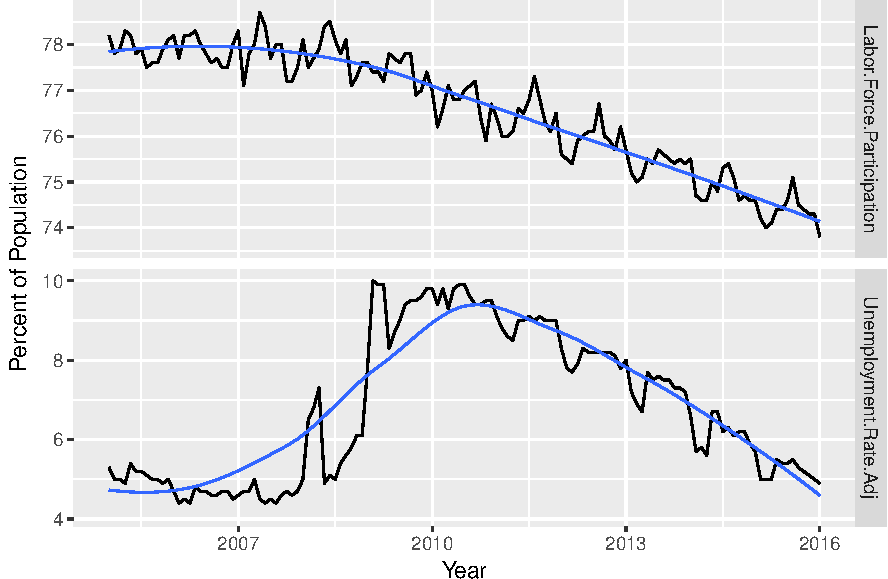
\includegraphics{elliott-econometric-personnel-retention-18_files/figure-latex/lfpr-unemployment-1} 

}

\caption{Participation and Unemployment}\label{fig:lfpr-unemployment}
\end{figure}

It is assumed that the skillsets of the target population (Air Force
officers) are most transferrable to those jobs covered by nonfarm
payrolls. Nonfarm is a category of the labor force that excludes
proprietors, private household employees, unincorporated
self-employment, unpaid volunteers, and farm employees
\cite{fred-nonfarm-2017}. Job quits are generally voluntary separations
and may reflect workers' willingness to leave the job; it may be that
the a higher propensity to volutarily leave a job translates to a
positive outlook on obtaining another and the economy as a whole.

The labor market momentum index compares current labor market conditions
to historical averages. A negative value indicates conditions below the
long-term average, and a positive value indicates favorable conditions.
The CPI examines the weighted average price of a basket of consumer
goods and services; it is used to estimate the cost of living. There is
some uncertainty involving employment in separation from the military,
so cost of living information may be especially important to the
retention decision as the military is excluded from CPI statistics.

By including these variables in a regression model and estimating their
effects on military attrition trends, this work seeks to capture
military members' perceptions of economic health and job prospects, and
use that information as a means to forecast Air Force officer attrition.

\begin{table}

\caption{\label{tab:econ-var}Selected Economic Indicators}
\centering
\resizebox{\linewidth}{!}{\begin{tabular}[t]{ll}
\toprule
\bfseries{Variable} & \bfseries{Description}\\
\midrule
Labor Market Momentum Index & Compares current market conditions to long-run average\\
CPI & Weighted average price of a basket of goods and services\\
Nonfarm Jobs Openings & Unfilled positions at the end of the month in the nonfarm sector\\
Real GDP per Capita & Measure of economic output per person, adjusted for inflation\\
Nonfarm Job Quits & Voluntary separations from jobs in the nonfarm sector\\
\addlinespace
Unemployment Rate & Percentage of unemployed individuals in the labor force\\
Labor Force Participation Rate & Percentage of the population either employed or actively seeking work\\
\bottomrule
\end{tabular}}
\end{table}

\hypertarget{cleaning-and-preparation}{%
\subsection{Cleaning and Preparation}\label{cleaning-and-preparation}}

Perfect data are rarely found or received outside of the classroom, and
such is the case here. Before exploration and modeling, several steps
helped produce a useable data set.

The personnel data is first converted from long to wide format.
Originally, the personnel data comes with three variables: Air Force
Specialty Code (AFSC), Date, and Separations. This form is not conducive
to modeling. A new variable is thus created for each category in AFSC
containing the associated separation counts. This procedure generates
missing values, which then must be dealt with appropriately. Missing
values can result from several underlying issues: data storage
corruption, entry errors, miscommunication between software, none of
which apply here. Since the attrition data is a monthly count of people
exiting USAF service, the intuition is that these missing values simply
represent a lack of an observation (i.e.~zero separations). This is
confirmed by the data's provider. Therefore all missing values in the
personnel data are replaced with zero. Initially, observation dates are
stored as the number of days since 1 Jan 1960 (the standard for SAS).
This is transformed into YYYY-MM-DD to facilitate its merging with the
economic data. An additional column is tabulated, the total separations
across all AFSCs. This column total is the response used for the
modeling efforts

The economic data do not require much treatment as they come from a
professionally managed database. One of the indicators, real GDP per
capita, occurs in quarterly intervals while the rest are monthly. To
make data comparable, the quarterly values are applied across each month
in the quarter (e.g.~the observation for Q1 2006 is applied over
January, Febuary, and March 2006). Then, variables are also renamed for
clarity. Finally, economic data are merged with the personnel data
through an inner join, preserving only those observations with dates
common to both data sets.

\hypertarget{model-selection}{%
\section{Model Selection}\label{model-selection}}

\hypertarget{introduction-2}{%
\subsection{Introduction}\label{introduction-2}}

General modeling practices involve horizontally splitting the original
data set into at least two, sometimes three, subsets. This ensures model
fitting and assessment are independent processes. There are many ways to
generate these subsets, each particular to the structure of the data.
With time-series data, as in this research, the typical approach is to
retain roughly the first 80 percent of the data for model fitting,
leaving the rest for model assessment. These two sections are
respectively known as the training and validation sets. The training set
is used to estimate model parameters, which are then used for
predictions on subsequent observations. These predictions are compared
against the validation set - actual, observed data - as a means of
assessing model performance. Model performance is assessed using three
criteria: the corrected Akaike Information Criteria (AICc), training
root mean square error (training RMSE), and validation root mean square
error (validation RMSE). Generally, better model performance is
associated with lower scores for each criteria, so `good' models are
identified by having lower scores relative to other models. The
training/validation approach is applied to each modeling technique
employed.

This endeavor utilizes two modeling techniques for forecasting:
na\textbackslash{}"ive models and dynamic regression models (also known
as transfer functions). The former is a far simpler technique and is
used as a baseline. The latter is a bit more complex. Dynamic regression
has two major components, regression and time-series, each with their
own assumptions and requirements.

Regression models with multiple predictor variables assume independence
of those predictors (also called regressors or exogeneous variables).
All regression models assume errors are normally and independently
distributed around zero with constant variance. The regression portion
is primarily concerned with coefficients of the predictor variables.
These coefficients provide insight as to which predictors have a
statisically significant effect in explaining the variability in the
data.

ARIMA models are used to address the pecularities of time series data,
and a brief review of those characteristics is necessary to understand
the analysis presented later in this chapter. Foremost is the concept of
autocorrelation, which is when a variable (e.g.~the temperature) depends
on previous observations of itself. Another concept central to
subsequent modeling efforts is that of stationarity. A stationary
variable is one that does not exhibit mean changes, such as caused by
trend or seasonality effects - when plotted over time. Stationarity is
requisite for generating reliable forecasts with time-series models.
Last is a matter of notation. In this work, backshift notation is used
to indicate backwards time steps, denoted with \(B\) and is defined
below:

For a single step back, \[ By_t = y_{t-1}, \] for two steps back,
\[ B^2y_t = y_{t-2}, \] and in general, \[ B^ky_t = y_{t-k}. \]

\hypertarget{initial-exploration}{%
\subsection{Initial Exploration}\label{initial-exploration}}

First, the data are examined visually. Plotting the response, total
separations over all career fields, in Figure \ref{fig:response-plot}
shows significant spikes during 2005, '06, '07, and '14. It is known
that during these periods, special spearation incentive programs were
introduced by th Air Fofce to artificially downsize the force. The
effects of these periods merit investigation later on, as they could
negatively affect model prediction performance.

\begin{figure}[H]

{\centering 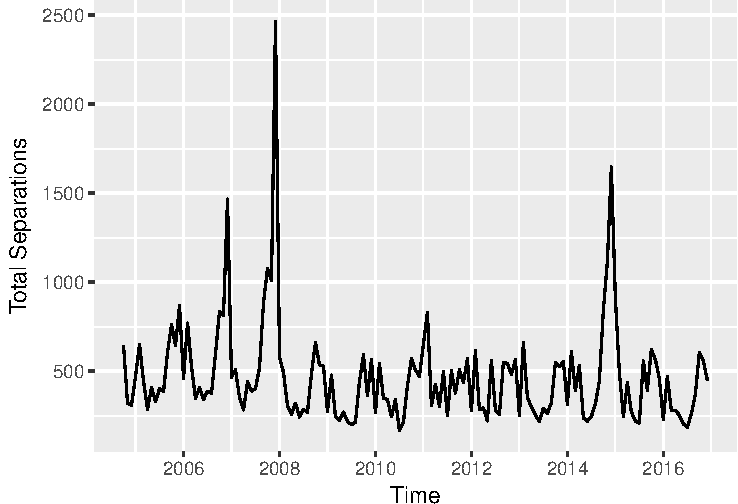
\includegraphics{elliott-econometric-personnel-retention-18_files/figure-latex/response-plot-1} 

}

\caption{Monthly Officer Separations}\label{fig:response-plot}
\end{figure}

No seasonality is immediately obvious in Figure \ref{fig:response-plot}.
However, if each year is plotted separately, a clearer picture emerges.
First, Figure \ref{fig:response-season-plot} shows that the extreme
points noticed noticed above seem to be relegated to the
November-December time frame. Second, it is easier to witness the
seasonality: bowing across the year, with higher counts at the beginning
and end.

\begin{figure}[H]

{\centering 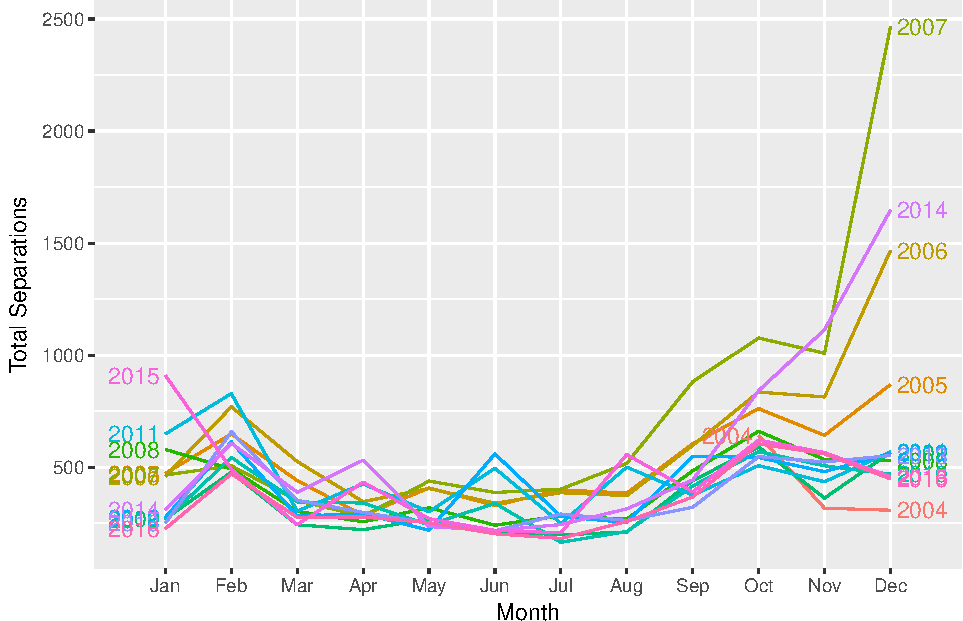
\includegraphics{elliott-econometric-personnel-retention-18_files/figure-latex/response-season-plot-1} 

}

\caption{Seasonal Plot: Total Separations}\label{fig:response-season-plot}
\end{figure}

Considering these plots, it is expected that a seasonal model performs
best and some alteration will have to be made to accomodate the
outliers. To confirm, na\textbackslash{}"ive models are fit to the data
and the results are examined. Beyond revealing seasonality and outlier
effects, fitting na\textbackslash{}"ive models establishes a baseline to
compare against later models. Na\textbackslash{}"ive models are very
simplistic, so if later models perform worse or only marginally better,
it implies they are not capturing much information.

Figure \ref{fig:n-sn-forecast} gives evidence to the negative effects of
outliers. Notice the large confidence intervals surrounding the
na\textbackslash{}"ive forecast and the 2014 spike carried through in
the seasonal forecast.

\begin{verbatim}
## <ScaleContinuousPosition>
##  Range:  
##  Limits:    0 --    1
\end{verbatim}

\begin{verbatim}
## <ScaleContinuousPosition>
##  Range:  
##  Limits:    0 --    1
\end{verbatim}

\begin{figure}[H]

{\centering 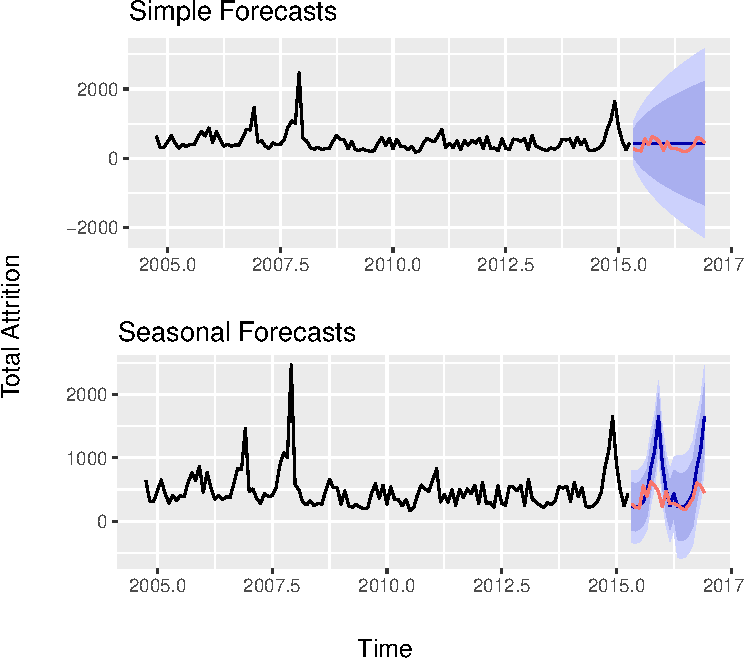
\includegraphics{elliott-econometric-personnel-retention-18_files/figure-latex/n-sn-forecast-1} 

}

\caption{Simple and Seasonal Na\"ive Forecasts}\label{fig:n-sn-forecast}
\end{figure}

Tables \ref{tab:n-err} and \ref{tab:sn-err} show different error metrics
for each of the two models. Judging by root mean square error (RMSE),
the seasonal model generally fits the training data better, possibily
indicating presence of seasonality effects. However, there is a large
disparity between validation RMSEs, possibly caused by the major spike
in 2014 - reaffirming the earlier intuition about outlier effects.

\begin{table}[!h]

\caption{\label{tab:n-err}Na\"ive Results}
\centering
\begin{tabular}[t]{lcccccc}
\toprule
\bfseries{ } & \bfseries{ME} & \bfseries{RMSE} & \bfseries{MAE} & \bfseries{MPE} & \bfseries{MAPE} & \bfseries{MASE}\\
\midrule
Training set & -1.651 & 312.523 & 195.984 & -12.530 & 42.093 & 1.261\\
Test set & -62.600 & 160.642 & 144.300 & -37.265 & 51.569 & 0.928\\
\bottomrule
\end{tabular}
\end{table}\begin{table}[!h]

\caption{\label{tab:sn-err}Seasonal Na\"ive Results}
\centering
\begin{tabular}[t]{lcccccc}
\toprule
\bfseries{ } & \bfseries{ME} & \bfseries{RMSE} & \bfseries{MAE} & \bfseries{MPE} & \bfseries{MAPE} & \bfseries{MASE}\\
\midrule
Training set & 16.496 & 291.791 & 155.452 & -7.374 & 30.452 & 1.000\\
Test set & -238.850 & 454.288 & 271.450 & -59.852 & 67.315 & 1.746\\
\bottomrule
\end{tabular}
\end{table}

It is known that during years 2005, '06, '07, and '14 special separation
programs were implemented. Given the effect those years appear to have
on modeling, they must be accomodated before continuing. Before deciding
how, the explicit points in question need to be identified. To help,
refer to Figure \ref{fig:response-season-plot}. As noted above, the
spikes generally occur in November and December. However, the
observations from 2005 are close enough to those from other years that
they may have resulted naturally. Minimal removal of information from
the data set is desired, removing only that which is misleading. So,
November and December observations from 2006, '07, and '14 are selected
for replacement.

Given the seasonality in the data set, the replaced values should stem
from matching observations in previous years, as opposed to previous
observations within the same year. The outliers are replaced (or
imputed) with the arithmetic mean of all years not being replaced
(e.g.~November 2006, '07, '14 are replaced with the mean separations in
November for all other years).

Replotting the response in Figure \ref{fig:response-plot-2} shows a much
better behaved data set. The data look fairly stationary, setting the
stage for developing more complex forecasting models.

\begin{figure}[H]

{\centering 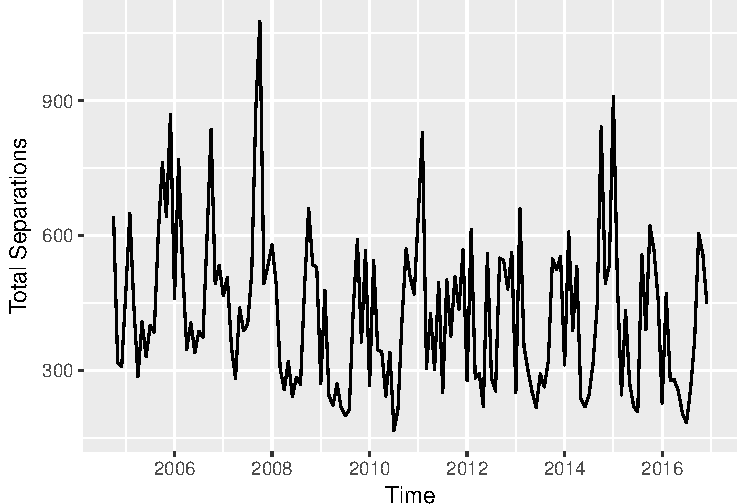
\includegraphics{elliott-econometric-personnel-retention-18_files/figure-latex/response-plot-2-1} 

}

\caption{Separations - Outliers Removed}\label{fig:response-plot-2}
\end{figure}

With the outliers replaced, seasonal effects are much more apparent (see
Figure \ref{fig:response-season-plot-2}), further enforcing the need for
a seasonal model.

\begin{figure}[H]

{\centering 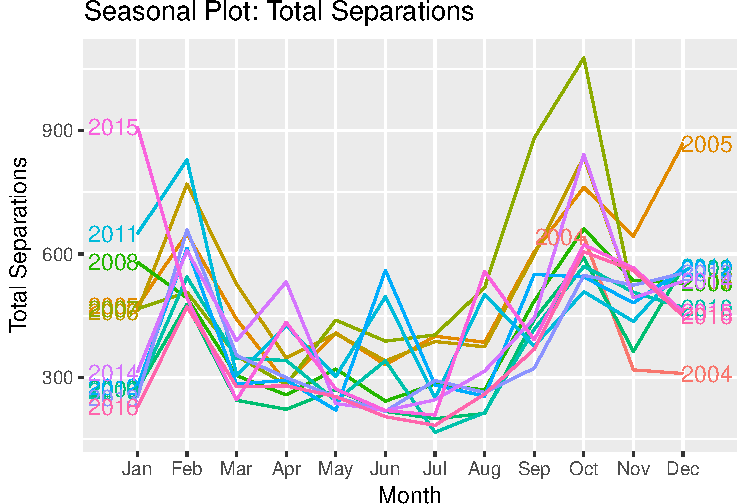
\includegraphics{elliott-econometric-personnel-retention-18_files/figure-latex/response-season-plot-2-1} 

}

\caption{Seasonal Plot: Outliers Removed}\label{fig:response-season-plot-2}
\end{figure}

Table \ref{tab:season-rmse-compare} compares the seasonal
na\textbackslash{}"ive RMSEs before and after imputing the identified
outliers. The results indicate that removing and replacing the extreme
values for November and December improved the model. This is further
reflected by the forecast (shown in blue) in Figure
\ref{fig:sn-forecast-2}, which follows the validation data (shown in
orange) more closely than those in Figure \ref{fig:n-sn-forecast}.
Overall, these results imply that imputation of the selected
observations was useful.

\begin{table}[!h]

\caption{\label{tab:season-rmse-compare}Seasonal Na\"ive RMSE Comparison}
\centering
\begin{tabular}[t]{lcc}
\toprule
\bfseries{ } & \bfseries{Raw Data} & \bfseries{Imputed Data}\\
\midrule
Training & 291.791 & 161.262\\
Validation & 454.288 & 186.584\\
\bottomrule
\end{tabular}
\end{table}

\begin{figure}[H]

{\centering 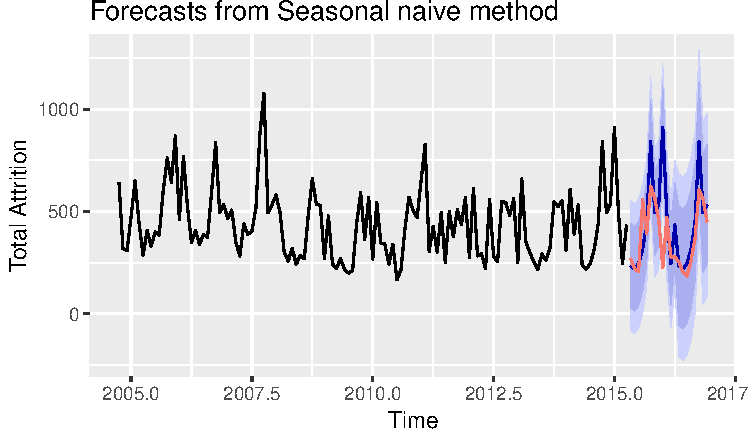
\includegraphics{elliott-econometric-personnel-retention-18_files/figure-latex/sn-forecast-2-1} 

}

\caption{Seasonal Na\"ive Forecast After Imputation}\label{fig:sn-forecast-2}
\end{figure}

\hypertarget{dynamic-regression}{%
\subsection{Dynamic Regression}\label{dynamic-regression}}

Na\textbackslash{}"ive models are simple, regression models adequately
involve exogenous predictor variables, and time series model adequately
handle autoregressive components of data. Individually these models are
useful, but cannot handle both exogenous and autoregressive components.

Dynamic regression is a regression model with an ARIMA model fit to the
errors. The regression piece allows use of independent variables in
predicting a response, and the ARIMA portion helps model the
autoregressive information which can exist in time-series data. The
general formulation of a dynamic regression model with ARIMA(1,1,1)
errors:

\[ y_t = \beta_0 + \beta_1x_{1,t} + ... + \beta_kx_{k,t} + n_t\] where,

\[ (1-\phi_1B)(1-B)n_t = (1+\theta_1B)e_t \] and \(e_t\) is white noise.
The \(\phi_1\) is the non-seasonal autoregressive coefficient while the
\(\theta_1\) is the non-seasonal moving average coefficient. The
\((1-B)\) indicates the errors are also subjected to a single order of
differencing to achieve a stationary time-series in the error term.

Fitting a dynamic regression model requires taking several steps to
ensure key assumptions are not violated. First is to address the issue
of collinearity. Collinearity between predictor variables implies a
dependent relationship and can lead to innaccurate coefficient
estimates, a result contrary to the goal of any modeling effort. To
avoid this pitfall, a correlation matrix of possible regressors is
compiled and examined. A correlation matrix shows how collinear each
pair of indicators is. A high correlation coefficient between indicators
implies collinearity, meaning the variables should not be used together
in the model. Figure \ref{fig:heat-map-1} shows the correlation between
all pair-wise combinations of variables in the economic data set. There
are many instances of collinearity, which is expected since many
economic indicators are constructed from similar information. There are
some independent subsets, though, and these are the candidates for the
dynamic regression model.

\begin{figure}[H]

{\centering 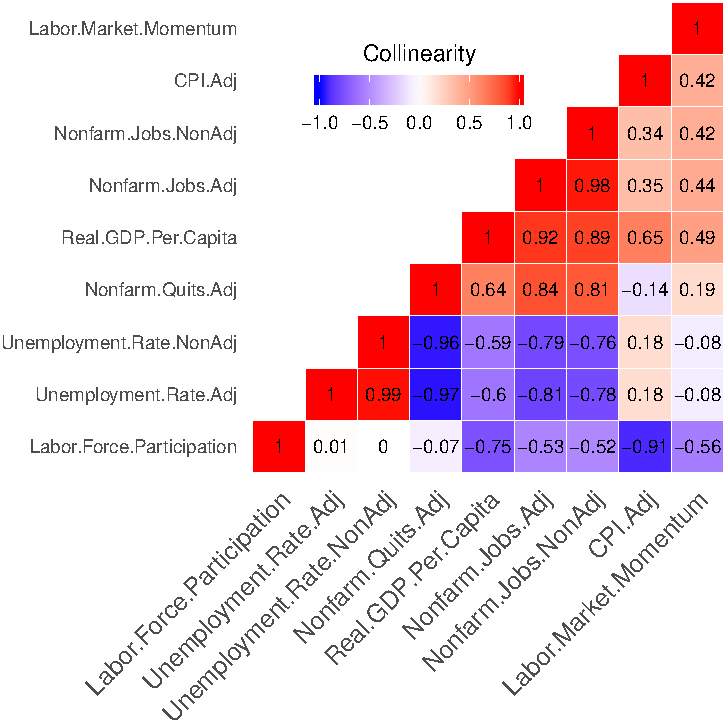
\includegraphics{elliott-econometric-personnel-retention-18_files/figure-latex/heat-map-1-1} 

}

\caption{Correlation Matrix - Economic Indicators}\label{fig:heat-map-1}
\end{figure}

Given their low correlation, Unemployment Rate (Adj.), Labor Force
Participation Rate, and Labor Market Momentum Index are selected as
independent variables. To ensure the assumptions made by the ARIMA piece
of the model, the stationarity of the regressors is checked. Though
trend and seasonality components can be incorporated through regression
techniques, ARIMA models require stationarity. Non-stationary variables
can produce inconsistent coefficient estimates, even if they are
independent. To assess, a plot of the three indicators in Figure
\ref{fig:econ-vars-1} is generated.

\begin{figure}[H]

{\centering 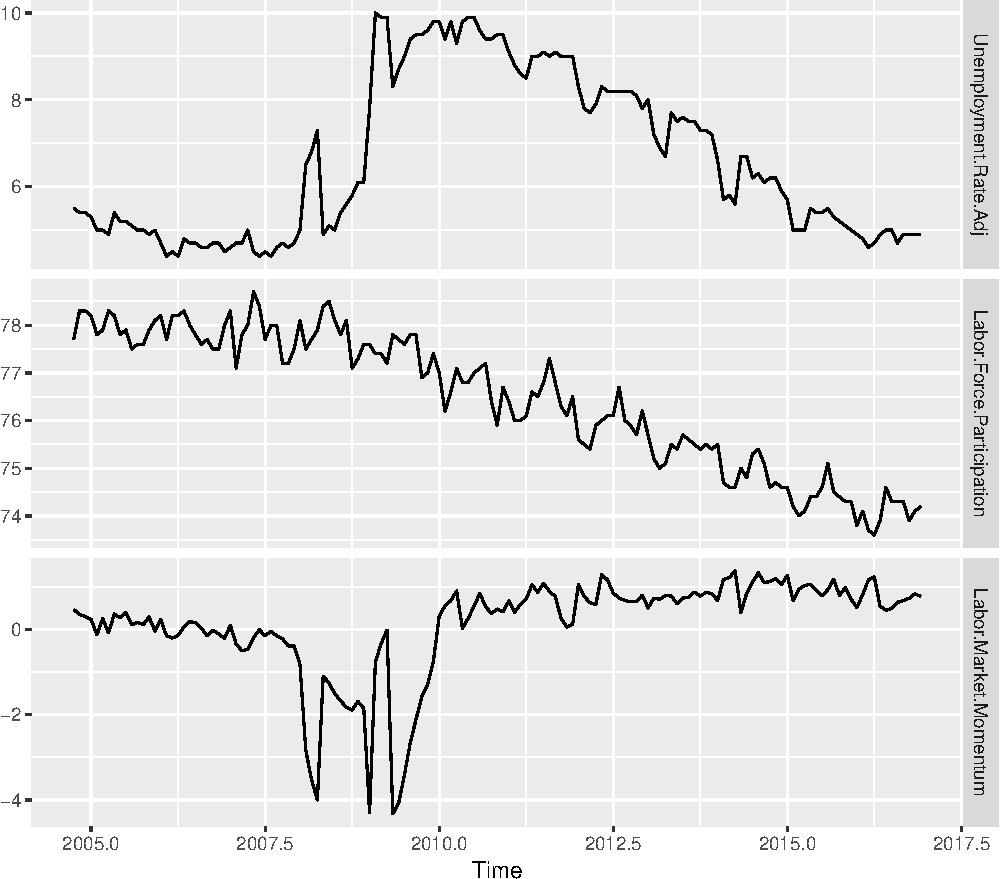
\includegraphics{elliott-econometric-personnel-retention-18_files/figure-latex/econ-vars-1-1} 

}

\caption{Economic Indicators - Raw}\label{fig:econ-vars-1}
\end{figure}

Each of the three indicators show evidence of a trend or changing
mean(i.e.~are non-stationary). To handle this, the data are differenced.
The resulting data are shown below in Figure \ref{fig:econ-vars-2}.

\begin{figure}[H]

{\centering 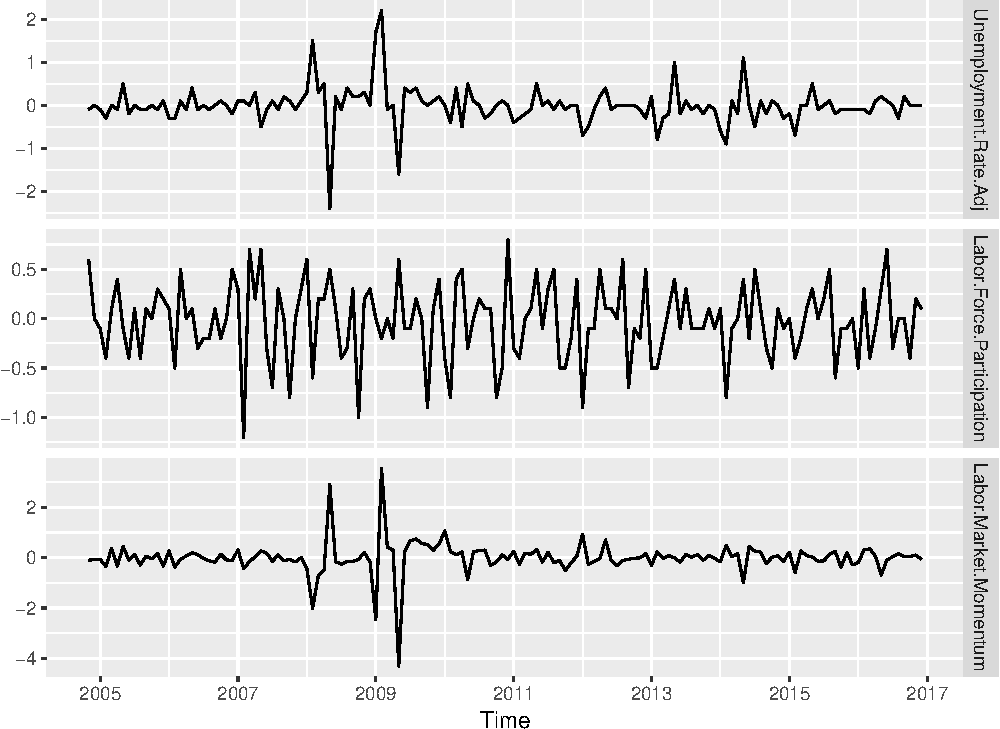
\includegraphics{elliott-econometric-personnel-retention-18_files/figure-latex/econ-vars-2-1} 

}

\caption{Economic Indicators - Differenced}\label{fig:econ-vars-2}
\end{figure}

Simple differencing produces the desired effect, the data are
stationary. It is important to note the regressors now show the
month-to-month change, which will be pertinent when interpreting
results.

With stationary and independent economic indicators, model formulation
can transition from regression to the ARIMA portion. Up to six
parameters can be specified and estimated: the order of autoregression,
degree of differencing, and order of the moving average (\(p,d,\) and
\(q\), respectively) and their seasonal counterparts (\(P,D,\) and
\(Q\)). Many combinations are considered. A range is specified for each
parameter, and a model is fit for every combination within the specified
ranges; the model with the lowest corrected Akaike Information Criteria
(AICc) is selected. For the first, and all subsequent, dynamic
regression models in this work, the following ranges/values were used:
\(p,q \in [0,5]\), \(d,D = 0\), and \(P, Q \in [0,2]\).

For this first pass, the model selected was a regression model with a
fourth-order moving average and first-order seasonal autoregression on
the errors. More explicitly:

\[ y = \beta_0 + \beta_1x'_{1,t} + \beta_2x'_{2,t} + \beta_3x'_{3,t} + n_t\]
where,
\[ (1-\Phi_1 B^{12})n_t = (1 + \theta_1B + \theta_2B^2 + \theta_3B^3 + \theta_4 B^4)e_t \]
and, \[ x'_{i,t} = x_{i,t} - x_{i,t-1}\] The coefficient estimates are
shown in Table \ref{tab:dynreg1-coeff}:

\begin{table}[!h]

\caption{\label{tab:dynreg1-coeff}Estimated Coefficients - Initial Model}
\centering
\begin{tabular}[t]{lccccccccc}
\toprule
\bfseries{ } & \bfseries{$\theta_1$} & \bfseries{$\theta_2$} & \bfseries{$\theta_3$} & \bfseries{$\theta_4$} & \bfseries{$\Phi_1$} & \bfseries{$\beta_0$} & \bfseries{$\beta_1$} & \bfseries{$\beta_2$} & \bfseries{$\beta_3$}\\
\midrule
Coeff & 0.218 & 0.145 & 0.336 & 0.260 & 0.576 & 429.875 & -13.390 & -15.949 & -2.819\\
StdErr & 0.087 & 0.088 & 0.092 & 0.092 & 0.082 & 47.602 & 22.286 & 35.016 & 11.494\\
\bottomrule
\end{tabular}
\end{table}

Model assessment involves analysis of the residuals. Residuals are
examined for evidence of remaining autocorrelation, satisfaction of
normality assumptions (\(e_t \sim N(0,\sigma^2)\)), and outlier effects.
Figure \ref{fig:dynreg1-resid} provides the plots used to answer those
questions. The top subfigure plots the raw model residuals, and is used
to identify possible trends, seasonality, or heteroscedasticity.
Fortunately, none of those features are apparent. The bottom-left is
used to examine significant autocorrelation in the residuals;
significant correlations would indicate a possible violation of the
independence of the residuals. The current model's results only show one
lag-period with significant autocorrelation, which may mean that there
is information unnaccounted for by the current model. Overall
autocorrelation, however, appears insignificant, as further evidenced by
the results of a Ljung-Box test for autocorrelation (Table
\ref{tab:dynreg1-boxtest}). The bottom-right plot shows a histogram of
the residuals, comparing the raw distribution against the ideal normal.
The plot shows slight skewness, but overall the data appear normal.
Thus, there is little, if any, misbehavior in the model's residuals.

\begin{figure}[H]

{\centering 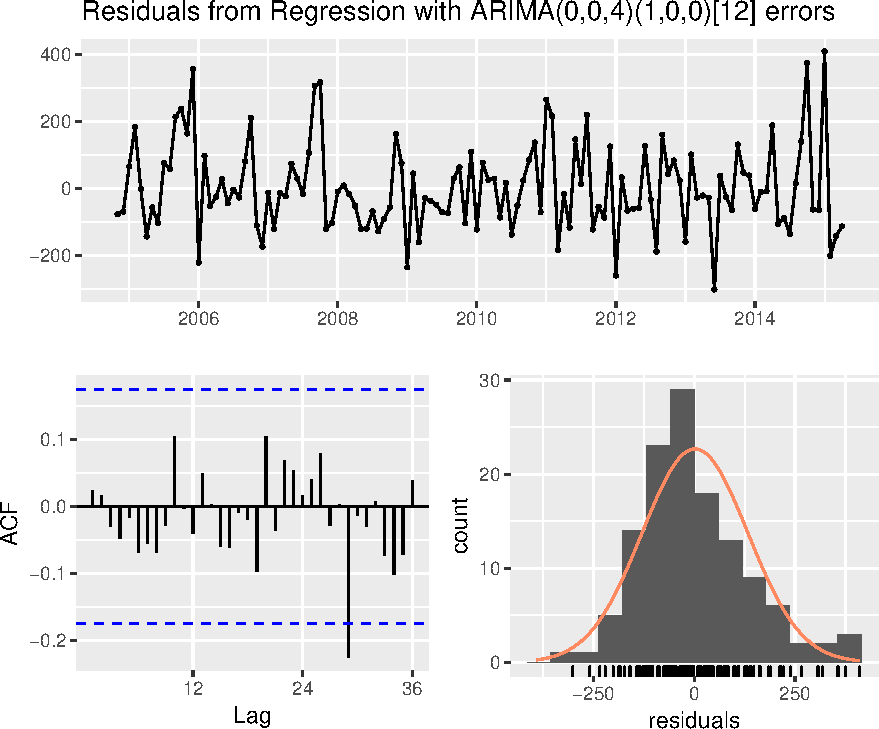
\includegraphics{elliott-econometric-personnel-retention-18_files/figure-latex/dynreg1-resid-1} 

}

\caption{Initial Attrition Model - Residual Analysis}\label{fig:dynreg1-resid}
\end{figure}

\begin{table}[!h]

\caption{\label{tab:dynreg1-boxtest}Initial Model - Autocorrelation Test}
\centering
\begin{tabular}[t]{lrr}
\toprule
\bfseries{Test type} & \bfseries{Test statistic} & \bfseries{p-value}\\
\midrule
Box-Ljung test & 10.121 & 0.812\\
\bottomrule
\end{tabular}
\end{table}

Forecasts are generated from the training data and compared against the
validation data. Figure \ref{fig:dynreg1-forecast} plots the training
and validation data against the model predictions. Large movements are
generally captured, even if not perfectly forecast. To compare modeling
performance, the RMSEs from the models are compared in Table
\ref{tab:model-compare-1}.

\begin{figure}[H]

{\centering 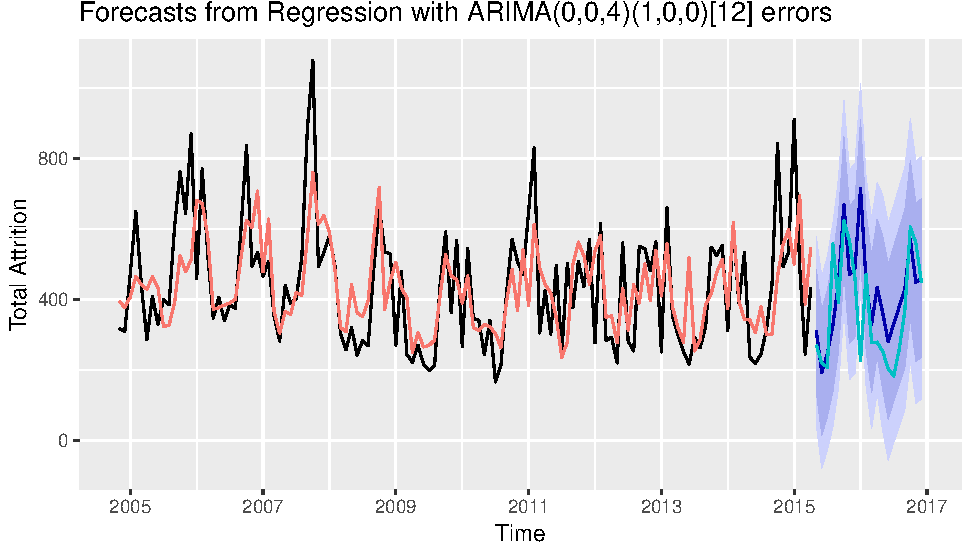
\includegraphics{elliott-econometric-personnel-retention-18_files/figure-latex/dynreg1-forecast-1} 

}

\caption{Initial Model - Forecasts Against Validation Data}\label{fig:dynreg1-forecast}
\end{figure}

\begin{table}[!h]

\caption{\label{tab:model-compare-1}Model RMSE Comparison}
\centering
\begin{tabular}[t]{lrrr}
\toprule
\bfseries{ } & \bfseries{Simple Na\textbackslash{}"ive} & \bfseries{Seasonal Na\textbackslash{}"ive} & \bfseries{Dynamic Regression}\\
\midrule
Training & 199.832 & 161.262 & 130.746\\
Validation & 160.642 & 186.584 & 142.988\\
\bottomrule
\end{tabular}
\end{table}

Dynamic regression demonstrates greater ability to forecast the
attrition data than the na\textbackslash{}"ive models. However, the high
standard errors of the regression coefficients (\(\beta_1\),
\(\beta_2\), and \(\beta_3\) in Table \ref{tab:dynreg1-coeff}) indicate
that none of the economic indicators are statistically significant. This
means the ARIMA model handles all the forecasting and the regression
provides little insight. Essentially, the economic predictor variables
do not explain much of the data variability. This could be for several
reasons:

\begin{itemize}
\item
  With differencing, the indicators represent month-to-month changes.
  For most observations in the data set those changes are marginal,
  resulting in an insignificant effect on attrition, at least
  numerically.
\item
  The economic and personnel data are both aggregated to the national
  level. It is possible that such a degree of aggregation includes
  enough noise to mask any economic effects.
\item
  As they are, the indicators show only the previous month's change. The
  regression coefficients represent the effects last month's changes
  have on this month's attrition. Intuitively, this does not seem
  correct. Voluntary separation from the military is a long,
  bureaucratic process; as such, it is more probable that members decide
  to leave the military more than a month ahead of time.
\end{itemize}

Unfortunately, there is not much that can be done about the first point.
As mentioned earlier, the indicators must be stationary in order to
ensure the reliability of any potential effects, and the data must be
differenced to be stationary.

\hypertarget{lagged-economic-indicators}{%
\subsection{Lagged Economic
Indicators}\label{lagged-economic-indicators}}

Occasionally with time-series data, the effect of one variable on
another is not be immediately observed. Consider a production firm
redirecting profit towards self-investment. Ideally, this investment
will lead to enhanced production capacity and higher revenue, though
likely at a much later date. In the same sense, the current economic
conditions could have a greater effect on attrition 12 months from now
than they do today. In this section, the relationships between attrition
and the lagged economic inidicators are explored.

The economic data is observed monthly over 12 years, and so there are
many possible lag-periods to consider. It is also possible that the best
lag-period is not identical for all predictors, so several combinations
of different predictors lagged to different periods should be tested.
This results in a very large test space. To decrease computational
requirements, lag-periods are restricted to 0, 6, 12, 18, and 24 months.
A separate dynamic regression model is generated for every combination
of predictor and lag-period. This amounts to 125 dynamic regression
models. The models are evaluated and compared on three metrics: AICc,
training RMSE, and validation RMSE. Any models that peform well by
comparison are inspected further.

Table \ref{tab:lag-results-1} below summarizes the values for each
performance metric. Note that the minimum value for each category are
below those seen in the previous model. This suggests that lagging the
model's predictors can yield better results than using current values.
The lagged models are thus invesitgated in greater detail.

\begin{table}[!h]

\caption{\label{tab:lag-results-1}Summary Statistics - Lag Results}
\centering
\begin{tabular}[t]{llll}
\toprule
\bfseries{ } & \bfseries{     AICc} & \bfseries{Training.RMSE} & \bfseries{Validation.RMSE}\\
\midrule
 & Min.   :1291 & Min.   :127.0 & Min.   :122.3\\
 & 1st Qu.:1299 & 1st Qu.:133.0 & 1st Qu.:156.3\\
 & Median :1372 & Median :134.8 & Median :163.9\\
 & Mean   :1361 & Mean   :134.6 & Mean   :164.8\\
 & 3rd Qu.:1378 & 3rd Qu.:137.7 & 3rd Qu.:175.1\\
 & Max.   :1613 & Max.   :140.4 & Max.   :187.6\\
\bottomrule
\end{tabular}
\end{table}

The 1st quartiles of each performance criteria are used to filter the
set of models, seeking models which perform well in all three
categories. Only one model does, when the unemployment rate is lagged by
24 months, labor force participation rate by 18 months, and labor market
momentum by 24 months.

\begin{table}[!h]

\caption{\label{tab:high-performers-1}High Performance Across All Criteria}
\centering
\begin{tabular}[t]{lllrrr}
\toprule
\bfseries{UR.lag} & \bfseries{LFPR.lag} & \bfseries{LMM.lag} & \bfseries{AICc} & \bfseries{Training.RMSE} & \bfseries{Validation.RMSE}\\
\midrule
lag24 & lag18 & lag24 & 1292.005 & 126.9902 & 146.6523\\
\bottomrule
\end{tabular}
\end{table}

Inspecting the model further reveals that one of the economic indicator
is a significant predictor, unemployment rate lagged at 24 months.
Unfortunately, none of the other predictors are significant in this
model (shown in Table \ref{tab:best-by-all-1}).

\begin{table}[!h]

\caption{\label{tab:best-by-all-1}Best Across All Criteria}
\centering
\begin{tabular}[t]{lrr}
\toprule
\bfseries{term} & \bfseries{estimate} & \bfseries{std.error}\\
\midrule
ma1 & -0.6686164 & 0.0993732\\
ma2 & -0.2256966 & 0.1119664\\
sar1 & 0.8797210 & 0.1779036\\
sma1 & -0.4942166 & 0.4519305\\
UR.lag.train[, "lag24"] & 83.5668948 & 24.7823250\\
\addlinespace
LFPR.lag.train[, "lag18"] & 66.5150439 & 35.9139704\\
LMM.lag.train[, "lag24"] & -2.3988843 & 13.6970392\\
\bottomrule
\end{tabular}
\end{table}

Top performers are also identified by comparing the best five models
from each criteria individually and looking for commonalities. The
results in Table \ref{tab:best-by-1} show that only AICc and Training
RMSE have commonalities. The models in common are where the unemployment
rate, labor force participation rate, and labor market momentum are
respectively lagged at (24, 18, 6), (24, 18, 18), and (24, 18, 24). The
identified models are next inspected individually for coefficient
significance.

\begin{table}[!h]

\caption{\label{tab:best-by-1}Common High Performers}
\centering
\begin{tabular}[t]{lllrrr}
\toprule
\bfseries{UR.lag} & \bfseries{LFPR.lag} & \bfseries{LMM.lag} & \bfseries{AICc} & \bfseries{Training.RMSE} & \bfseries{Validation.RMSE}\\
\midrule
\addlinespace[0.3em]
\multicolumn{6}{l}{\textbf{Best by AICc}}\\
\hspace{1em}lag24 &\vphantom{1} lag18 & lag6 & 1290.809 & 128.5034 & 164.7404\\
\hspace{1em}lag24 &\vphantom{1} lag18 & lag18 & 1290.939 & 128.5950 & 163.3188\\
\hspace{1em}lag24 & lag18 & lag12 & 1291.484 & 128.9926 & 165.1801\\
\hspace{1em}lag24 & lag18 & lag0 & 1291.670 & 129.1358 & 163.8772\\
\hspace{1em}lag24 &\vphantom{1} lag18 & lag24 & 1292.005 & 126.9902 & 146.6523\\
\addlinespace[0.3em]
\multicolumn{6}{l}{\textbf{Best by Training RMSE}}\\
\hspace{1em}lag24 & lag18 & lag24 & 1292.005 & 126.9902 & 146.6523\\
\hspace{1em}lag24 & lag24 & lag12 & 1292.050 & 128.2139 & 175.2866\\
\hspace{1em}lag24 & lag24 & lag6 & 1292.106 & 128.3596 & 171.1853\\
\hspace{1em}lag24 & lag18 & lag6 & 1290.809 & 128.5034 & 164.7404\\
\hspace{1em}lag24 & lag18 & lag18 & 1290.939 & 128.5950 & 163.3188\\
\addlinespace[0.3em]
\multicolumn{6}{l}{\textbf{Best by Validation RMSE}}\\
\hspace{1em}lag0 & lag0 & lag24 & 1306.135 & 135.0200 & 122.3425\\
\hspace{1em}lag0 & lag6 & lag0 & 1528.092 & 133.3393 & 134.2465\\
\hspace{1em}lag0 & lag0 & lag6 & 1527.850 & 133.2320 & 136.0557\\
\hspace{1em}lag6 & lag6 & lag6 & 1528.026 & 133.2758 & 138.7995\\
\hspace{1em}lag6 & lag0 & lag6 & 1528.028 & 133.3174 & 138.8589\\
\bottomrule
\end{tabular}
\end{table}

The last common model (24, 18, 24) has already been inspected; it is the
same one in Table \ref{tab:best-by-all-1}. That leaves two models for
comparison (24, 18, 6) and (24, 18, 18). Their coefficients are
summarized in Tables \ref{tab:common-1} and \ref{tab:common-2} below,
respectively. Both tables show similar results as the previous model
(24, 18, 24): The unemployment rate is a significant predictor, labor
force particpation has a large effect but with high standard error, and
labor market momentum has a small effect with a large standard error.

\begin{table}[!h]

\caption{\label{tab:common-1}Common High Performer 1}
\centering
\begin{tabular}[t]{lrr}
\toprule
\bfseries{term} & \bfseries{estimate} & \bfseries{std.error}\\
\midrule
ma1 & -0.6988796 & 0.0973710\\
ma2 & -0.2255698 & 0.1092249\\
sar1 & 0.6372280 & 0.0883485\\
UR.lag.train[, "lag24"] & 92.7925361 & 26.0922804\\
LFPR.lag.train[, "lag18"] & 60.2058317 & 35.8537777\\
LMM.lag.train[, "lag6"] & 10.9102055 & 11.7262875\\
\bottomrule
\end{tabular}
\end{table}

\begin{table}[!h]

\caption{\label{tab:common-2}Common High Performer 2}
\centering
\begin{tabular}[t]{lrr}
\toprule
\bfseries{term} & \bfseries{estimate} & \bfseries{std.error}\\
\midrule
ma1 & -0.6768423 & 0.0997710\\
ma2 & -0.2515895 & 0.1139329\\
sar1 & 0.6368839 & 0.0873641\\
UR.lag.train[, "lag24"] & 93.4916257 & 25.9975212\\
LFPR.lag.train[, "lag18"] & 61.6302177 & 35.3374730\\
LMM.lag.train[, "lag18"] & -10.2948441 & 11.9100709\\
\bottomrule
\end{tabular}
\end{table}

Recall in Figure \ref{fig:heat-map-1} that labor market momentum and
labor force particpation rate are moderately correlated. Investigation
into labor market momentum reveals that it is a combination of many
economic indicators, including labor force participation. In short,
labor market momentum repeats the information represented by the other
two predictors and could be introducing multicollinearity issues. Given
that information and the collection of estimates discussed above, labor
market momentum is removed.

Lagged variable analyis is repeated with labor market momentum excluded
from the list of possible predictors. 25 dynamic regression models are
generated (with the identical lag periods) and compared. This time, no
model falls under the 1st quartile for all performance criteria.
Comparing the top five performers for each criteria does yield results.
A dynamic regression model with the unemployment rate lagged by 24
months and labor force participation rate lagged by 18 months falls into
the top five performers under AICc and Training RSME. Notice that the
repsective lag periods are identical to those in earlier models. Table
\ref{tab:reduced-1} summarizes the coefficient estimates.

\begin{table}[!h]

\caption{\label{tab:reduced-1}Top Model - Reduced Model}
\centering
\begin{tabular}[t]{lrr}
\toprule
\bfseries{term} & \bfseries{estimate} & \bfseries{std.error}\\
\midrule
ma1 & -0.6951414 & 0.0974040\\
ma2 & -0.2326008 & 0.1099844\\
sar1 & 0.6315523 & 0.0887194\\
UR.lag.train[, "lag24"] & 93.0157912 & 26.2632321\\
LFPR.lag.train[, "lag18"] & 62.4380155 & 35.8104021\\
\bottomrule
\end{tabular}
\end{table}

Unfortunately, earlier trends in coefficient estimates hold. The
unemployment rate has a noticeable and significant effect, and the labor
force participation rate does not. It is worth mentioning, however, that
the coefficient estimates are very close to those in earlier models,
implying that labor market momentum is a redundant predictor. While
these models provide some evidence of significant effects, it is
possible that other combinations of economic indicators are better fit.
In the next section, this idea is explored.

\hypertarget{alternative-economic-subsets}{%
\subsection{Alternative Economic
Subsets}\label{alternative-economic-subsets}}

Section 3.2.3 notes that there exist other subsets of economic
indicators with low correlation, besides unemployment, labor force
participation, and labor market momentum. In particular, nonfarm job
quits and labor force particpation have a correlation coefficient of
-0.07, the next lowest after unemployment and labor force participation.
This motivates examination of dynamic regression models which include
the former pair. The models are generated and analyzed. Each predictor
is lagged at 0, 6, 12, 18, and 24 months, and a dynamic regression model
is produced for every combination. These models are compared by AICc,
training RMSE, and validation RMSE, seeking to identify top performers.

From this analysis, only one model produces results comparable to
previous models. Table \ref{tab:alt-indicators-1} displays the specified
model and its perfomance scores. Though the scores are marginally worse
than the best models from the previous iteration, the coefficient
estimates are more important in providing insight about attrition.

\begin{table}[!h]

\caption{\label{tab:alt-indicators-1}Alternative Predictors - Best Model}
\centering
\begin{tabular}[t]{llrrr}
\toprule
\bfseries{Quits.lag} & \bfseries{LFPR.lag} & \bfseries{AICc} & \bfseries{Training.RMSE} & \bfseries{Validation.RMSE}\\
\midrule
lag24 & lag24 & 1301.586 & 137.252 & 192.0631\\
\bottomrule
\end{tabular}
\end{table}

Unfortuntely, Table \ref{tab:alt-indicators-2} shows no evidence that
either predictor is statistically significant. The combination of labor
force participation and nonfarm quits does not affect attrition. As with
the intitial models, predictive capacity is likely managed by the ARIMA
portion alone.

\begin{table}[!h]

\caption{\label{tab:alt-indicators-2}Alternative Predictors - Coefficient Estimates}
\centering
\begin{tabular}[t]{lrr}
\toprule
\bfseries{term} & \bfseries{estimate} & \bfseries{std.error}\\
\midrule
ma1 & -0.8384799 & 0.0956497\\
sar1 & 0.7041322 & 0.0841965\\
Quits.lag.train[, "lag24"] & -0.1078249 & 0.0741378\\
LFPR.lag.train[, "lag24"] & 63.5418324 & 43.4367079\\
\bottomrule
\end{tabular}
\end{table}

\hypertarget{summary-of-analysis}{%
\subsection{Summary of Analysis}\label{summary-of-analysis}}

This section analysed nine economic indicators and hundreds of models,
in several iterations. The best models were identified and explored,
revealing some trends and signifcant predictors. The insights gleaned
from this process are summarized and discussed in the next chapter.

\newpage

\hypertarget{conclusions-and-insights}{%
\chapter{Conclusions and Insights}\label{conclusions-and-insights}}

The research sought to identify economic indicators with statistically
significant effects on attrition and to specify a mathematical model
with which to build reliable forecasts of attrition. Regarding the
former, nine separate economic indicators were initially considered
(summarized in Table \ref{tab:econ-var}). Correlation analysis was used
to identify subsets of variables exhibiting the least interdependence to
avoid the effects of multicollinearity. Initial modeling found no
statistically significant effects. However, subsequent attempts found
that lagged economic indicators were significant. Specifically, the
unemployment rate lagged by 24 months was found to be statistically
signifcant in all of the top performing models. No other variables
analyzed (labor market momentum, labor force participation, and nonfarm
job quits) showed evidence of significant effects. Regarding forecasting
capacity, all of the top performing dynamic regression models explored
in Chapter III exhibited lower training and validation RMSE than the
na\textbackslash{}"ive models. That is, the dynamic regression
technique, regardless of predictor significance, is better adapted for
forecasting attrition than simply applying previous observations
forward. This work confirms results found in previous endeavors (such as
Jantscher \cite{jantscher-2016}), reinforcing the relevance of the
unemployment rate to attrition. This work builds on that knowledge by
also providing a timeline, finding evidence that the current
unemployment rate has a significant effect on attrition two years later.

Many possibilites were addressed in this work; four
na\textbackslash{}"ive models and 33,792 unique dynamic regression
models (176 regression specifications, each with 192 ARIMA variations).
By no means does this encapsulate the total set of possible models.
There are many avenues left unexplored by this research. Future work in
this area could, first, explore different subsets of the economic
indicators identified. The initial set of economic indicators can also
easily be expanded; the relevant data is freely accessible to the
public. Only five unique lag-periods were investigated, and the
procedure discussed could easily incorporate more vaired time lags (at
the cost of more time and computational complexity). Lastly, all data
considered were aggregated to the national level and only total
attrition across U.S. Air Force officers was evaluated. Future work in
this area could, and should, investigate possible differences across
AFSC groupings and, if possible, at a higher level of fidelity
(e.g.~state or county vs.~national aggregates).

\newpage

\hypertarget{appendix-a.-r-code}{%
\chapter*{Appendix A. R Code}\label{appendix-a.-r-code}}
\addcontentsline{toc}{chapter}{Appendix A. R Code}

\tiny

\begin{Shaded}
\begin{Highlighting}[]
\CommentTok{# check for req'd packages, install if not present}
\NormalTok{list.of.packages <-}\StringTok{ }\KeywordTok{c}\NormalTok{(}\StringTok{"tidyverse"}\NormalTok{, }\StringTok{"lubridate"}\NormalTok{, }\StringTok{"sas7bdat"}\NormalTok{, }\StringTok{"fpp2"}\NormalTok{, }\StringTok{"reshape2"}\NormalTok{,}
                      \StringTok{"stargazer"}\NormalTok{, }\StringTok{"knitcitations"}\NormalTok{, }\StringTok{"RefManageR"}\NormalTok{, }\StringTok{"xtable"}\NormalTok{, }
                      \StringTok{"kableExtra"}\NormalTok{, }\StringTok{"zoo"}\NormalTok{, }\StringTok{"tictoc"}\NormalTok{)}
\NormalTok{new.packages <-}\StringTok{ }\NormalTok{list.of.packages[}\OperatorTok{!}\NormalTok{(list.of.packages }\OperatorTok\StringTok{ }\KeywordTok{installed.packages}\NormalTok{()[,}\StringTok{"Package"}\NormalTok{])]}
\ControlFlowTok{if}\NormalTok{(}\KeywordTok{length}\NormalTok{(new.packages)) }\KeywordTok{install.packages}\NormalTok{(new.packages, }\DataTypeTok{repos=}\StringTok{"http://cran.us.r-project.org"}\NormalTok{)}

\CommentTok{#library loadout}
\KeywordTok{library}\NormalTok{(sas7bdat)}
\KeywordTok{library}\NormalTok{(zoo)}
\KeywordTok{library}\NormalTok{(lubridate)}
\KeywordTok{library}\NormalTok{(reshape2)}
\KeywordTok{library}\NormalTok{(kableExtra)}
\KeywordTok{library}\NormalTok{(knitr)}
\KeywordTok{library}\NormalTok{(gridExtra)}
\KeywordTok{library}\NormalTok{(tictoc)}
\KeywordTok{library}\NormalTok{(tidyverse)}
\KeywordTok{library}\NormalTok{(fpp2)}


\CommentTok{# set directory for lazy data referencing - allow switch between macOS and Windows}
\CommentTok{# Basically just set working directory to wherever local repo is held}
\CommentTok{#setwd("~/Documents/Grad School/Thesis/github/afit.thesis/")}
\CommentTok{#setwd("C:/Users/Jake Elliott/Desktop/afit.thesis/")}

\CommentTok{#auto redirect working directory to file's location}
\KeywordTok{setwd}\NormalTok{(}\KeywordTok{dirname}\NormalTok{(}\KeywordTok{sys.frame}\NormalTok{(}\DecValTok{1}\NormalTok{)}\OperatorTok{$}\NormalTok{ofile))}

\CommentTok{# source file containing functions created for this analysis}
\CommentTok{#source("~/Documents/Grad School/Thesis/github/afit.thesis/custom-functions.R")}
\CommentTok{#source("C:/Users/Jake Elliott/Desktop/afit.thesis/custom-functions.R")}

\CommentTok{#auto redirect working directory to function file's location}
\KeywordTok{source}\NormalTok{(}\KeywordTok{paste0}\NormalTok{(}\KeywordTok{dirname}\NormalTok{(}\KeywordTok{sys.frame}\NormalTok{(}\DecValTok{1}\NormalTok{)}\OperatorTok{$}\NormalTok{ofile), }\StringTok{"/custom-functions.R"}\NormalTok{))}


\NormalTok{###################}
\CommentTok{#   Import Data   #}
\NormalTok{###################}

\CommentTok{# Personnel data}
\CommentTok{# simple list of AFSCs and description}
\NormalTok{afsc_list <-}\StringTok{ }\KeywordTok{read.sas7bdat}\NormalTok{(}\StringTok{"Data/lu_ao_afs.sas7bdat"}\NormalTok{)}
\CommentTok{# monthly records of assigned levels, broken out by AFSC - currently in longform}
\NormalTok{assigned <-}\StringTok{ }\KeywordTok{read.sas7bdat}\NormalTok{(}\StringTok{"Data/assigned_levels.sas7bdat"}\NormalTok{) }\OperatorTok\StringTok{ }
\StringTok{  }\KeywordTok{spread}\NormalTok{(AFS, Assigned)}
\CommentTok{# monthly separation counts, broken out by AFSC - currently in longform}
\NormalTok{attrition <-}\StringTok{ }\KeywordTok{read.sas7bdat}\NormalTok{(}\StringTok{"Data/separations_count.sas7bdat"}\NormalTok{) }\OperatorTok\StringTok{ }
\StringTok{  }\KeywordTok{spread}\NormalTok{(AFS, Separation_Count) }

\CommentTok{# Econ data}
\KeywordTok{setwd}\NormalTok{(}\StringTok{"Data"}\NormalTok{)}
\NormalTok{econ_data <-}\StringTok{ }\KeywordTok{list.files}\NormalTok{(}\DataTypeTok{pattern =} \StringTok{"*_natl.csv"}\NormalTok{) }\OperatorTok\StringTok{ }
\StringTok{  }\CommentTok{# Import data sets}
\StringTok{  }\KeywordTok{lapply}\NormalTok{(read_csv) }\OperatorTok\StringTok{ }
\StringTok{  }\CommentTok{# Merge all sets }
\StringTok{  }\KeywordTok{Reduce}\NormalTok{(}\ControlFlowTok{function}\NormalTok{(x,y) }\KeywordTok{merge}\NormalTok{(x, y, }\DataTypeTok{by =} \StringTok{"DATE"}\NormalTok{), .) }\OperatorTok\StringTok{ }
\StringTok{  }\CommentTok{# Store data as tibble}
\StringTok{  }\KeywordTok{as.tibble}\NormalTok{() }

\CommentTok{# Now, because gdp per cap is observed only on a quarterly basis, we add it separately}
\CommentTok{# in order to handle the missing values resulting from a merge. This merge is }
\CommentTok{# from the previous in that it keeps all values from the existing data set, creating NAs}
\CommentTok{# where gdp_per_cap does not match with other observations. Merging the quarterly }
\CommentTok{# gdp_per_cap data with the monthly indicators results in NAs in gdp_per_cap where }
\CommentTok{# the dates do not match. We then handle NAs by extending the quarterly records throughout }
\CommentTok{# their respective quarters (e.g. the GDP per cap for Q1 2014 is applied to Jan-Mar 2014).}
\CommentTok{# Simultaneously, we will rename the variables for interpretability.}

\CommentTok{# Read in GDP per capita}
\NormalTok{gdp_per_cap <-}\StringTok{ }\KeywordTok{read_csv}\NormalTok{(}\StringTok{"real09_gdp_percap.csv"}\NormalTok{)}
\CommentTok{# Combine gdp per cap with econ_data, using a left-join (all.x = TRUE) to preserve the main data set}
\NormalTok{econ_data <-}\StringTok{ }\KeywordTok{merge}\NormalTok{(econ_data, gdp_per_cap, }\DataTypeTok{by =} \StringTok{"DATE"}\NormalTok{, }\DataTypeTok{all.x =} \OtherTok{TRUE}\NormalTok{) }\OperatorTok
\StringTok{  }\KeywordTok{as.tibble}\NormalTok{() }\OperatorTok
\StringTok{  }\CommentTok{# Rename column headers to something more meaningful}
\StringTok{  }\KeywordTok{select}\NormalTok{(}\DataTypeTok{Unemployment.Rate.Adj =}\NormalTok{ UNRATE, }\DataTypeTok{Unemployment.Rate.NonAdj =}\NormalTok{ UNRATENSA,}
         \DataTypeTok{CPI.Adj =}\NormalTok{ CPIAUCSL, }\DataTypeTok{Nonfarm.Jobs.Adj =}\NormalTok{ JTSJOL, }
         \DataTypeTok{Nonfarm.Jobs.NonAdj =}\NormalTok{ JTUJOL, }\DataTypeTok{Labor.Force.Participation =}\NormalTok{ LNS11327662, }
         \DataTypeTok{Labor.Market.Momentum =}\NormalTok{ FRBKCLMCIM, }\DataTypeTok{Real.GDP.Per.Capita =}\NormalTok{ A939RX0Q048SBEA, }
         \DataTypeTok{Nonfarm.Quits.Adj =}\NormalTok{ JTSQUL, }\DataTypeTok{Date =}\NormalTok{ DATE)}

\CommentTok{# The na.locf() command below carries a value forward through NAs until the next non-empty value is met; }
\CommentTok{# this is how we choose to represent the gdp per capita through an entire quarter}
\NormalTok{econ_data}\OperatorTok{$}\NormalTok{Real.GDP.Per.Capita <-}\StringTok{ }\KeywordTok{as.numeric}\NormalTok{(econ_data}\OperatorTok{$}\NormalTok{Real.GDP.Per.Capita) }\OperatorTok\StringTok{ }
\StringTok{  }\KeywordTok{na.locf}\NormalTok{()}


\NormalTok{#######################################}
\CommentTok{#   Data Cleaning and Preparation     #}
\NormalTok{#######################################}

\CommentTok{# The dates in the personnel data are in total days since 1 Jan 1960 (SAS default)}
\CommentTok{# We'll need to reformat the date into something readable and mergeable with our }
\CommentTok{# econ set. Also, we create a new column - the total number of separations across }
\CommentTok{# all AFSCs. We'll also create totals for different categories of officers: rated, }
\CommentTok{# non-rated, line, etc.}
\NormalTok{attrition <-}\StringTok{ }\KeywordTok{mutate}\NormalTok{(attrition, }\DataTypeTok{Total =} \KeywordTok{rowSums}\NormalTok{(attrition[}\OperatorTok{-}\DecValTok{1}\NormalTok{], }\DataTypeTok{na.rm =} \OtherTok{TRUE}\NormalTok{)) }\OperatorTok\StringTok{ }
\StringTok{  }\KeywordTok{mutate}\NormalTok{(}\DataTypeTok{temp =}\NormalTok{ EOP_Date }\OperatorTok{*}\StringTok{ }\DecValTok{86400}\NormalTok{) }\OperatorTok\StringTok{ }
\StringTok{  }\KeywordTok{mutate}\NormalTok{(}\DataTypeTok{Date =} \KeywordTok{as.POSIXct}\NormalTok{(temp, }\DataTypeTok{origin =} \StringTok{"1960-01-01"}\NormalTok{)) }\OperatorTok\StringTok{ }
\StringTok{  }\KeywordTok{within}\NormalTok{(}\KeywordTok{rm}\NormalTok{(temp, EOP_Date))}

\CommentTok{# repeat prodcedure for assigned data}
\NormalTok{assigned <-}\StringTok{ }\KeywordTok{mutate}\NormalTok{(assigned, }\DataTypeTok{Total =} \KeywordTok{rowSums}\NormalTok{(assigned[}\OperatorTok{-}\DecValTok{1}\NormalTok{], }\DataTypeTok{na.rm =} \OtherTok{TRUE}\NormalTok{)) }\OperatorTok\StringTok{ }
\StringTok{  }\KeywordTok{mutate}\NormalTok{(}\DataTypeTok{temp =}\NormalTok{ EOP_Date }\OperatorTok{*}\StringTok{ }\DecValTok{86400}\NormalTok{) }\OperatorTok\StringTok{ }
\StringTok{  }\KeywordTok{mutate}\NormalTok{(}\DataTypeTok{Date =} \KeywordTok{as.POSIXct}\NormalTok{(temp, }\DataTypeTok{origin =} \StringTok{"1960-01-01"}\NormalTok{)) }\OperatorTok\StringTok{ }
\StringTok{  }\KeywordTok{within}\NormalTok{(}\KeywordTok{rm}\NormalTok{(temp, EOP_Date))}

\CommentTok{# However, the date variables differ slightly between the econ and personnel sets:}
\CommentTok{# Though both represent monthly observations, the econ set default to the first }
\CommentTok{# of each month, and the personnel data defaulted to the last }
\CommentTok{# (e.g. October 2004 is represented as 01-10-2004 in the former, and 31-10-2004 in the latter)}
\CommentTok{# To handle this, we'll create new date variables in each set that have the days }
\CommentTok{# trimmed off, then merge. Merging isn't strictly necessary, but it is a convenient}
\CommentTok{# way to only keep those observations common to both data sets.}
\NormalTok{econ_data <-}\StringTok{ }\KeywordTok{mutate}\NormalTok{(econ_data, }\StringTok{"Date1"}\NormalTok{ =}\StringTok{ }\KeywordTok{paste}\NormalTok{(}\KeywordTok{year}\NormalTok{(Date), }\KeywordTok{month}\NormalTok{(Date)))}
\NormalTok{attrition <-}\StringTok{ }\KeywordTok{mutate}\NormalTok{(attrition, }\StringTok{"Date1"}\NormalTok{ =}\StringTok{ }\KeywordTok{paste}\NormalTok{(}\KeywordTok{year}\NormalTok{(Date), }\KeywordTok{month}\NormalTok{(Date)))}
\CommentTok{# Merge data sets}
\NormalTok{df <-}\StringTok{ }\KeywordTok{merge}\NormalTok{(econ_data, attrition, }\DataTypeTok{by =} \StringTok{"Date1"}\NormalTok{)}

\CommentTok{# Next, we see many NAs within the attrition data set. Given the data's nature, }
\CommentTok{# our intuition was that these missing values aren't a result of encoding error }
\CommentTok{# or similar, but rather an indication that no separations occurred during }
\CommentTok{# that period (i.e. NAs indicate no separations were observed, instead of}
\CommentTok{# indicating some sort of error). This intuition was confirmed by the data's}
\CommentTok{# provider, HAF/A1FPX.}
\NormalTok{df[}\KeywordTok{is.na}\NormalTok{(df)] <-}\StringTok{ }\DecValTok{0}

\CommentTok{# Next we'll go ahead and drop all of our date variables. When we use df}
\CommentTok{# to create a time series object, the date variables become redundant.}
\NormalTok{df <-}\StringTok{ }\NormalTok{df[, }\OperatorTok{!}\NormalTok{(}\KeywordTok{names}\NormalTok{(df) }\OperatorTok\StringTok{ }\KeywordTok{c}\NormalTok{(}\StringTok{"Date1"}\NormalTok{, }\StringTok{"Date.x"}\NormalTok{, }\StringTok{"Date.y"}\NormalTok{))]}

\CommentTok{# Now we'll initialize the time series object - start = Oct 2004, freq = 12 - }
\CommentTok{# and create the validation and training sets. Since we're only really interested}
\CommentTok{# in the Total column for modeling purposes}
\NormalTok{df.ts}\FloatTok{.1}\NormalTok{ <-}\StringTok{ }\KeywordTok{ts}\NormalTok{(df, }\DataTypeTok{start =} \KeywordTok{c}\NormalTok{(}\DecValTok{2004}\NormalTok{, }\DecValTok{10}\NormalTok{), }\DataTypeTok{frequency =} \DecValTok{12}\NormalTok{)}
\NormalTok{train.ts}\FloatTok{.1}\NormalTok{ <-}\StringTok{ }\KeywordTok{subset}\NormalTok{(df.ts}\FloatTok{.1}\NormalTok{, }\DataTypeTok{end =} \DecValTok{127}\NormalTok{)}
\NormalTok{val.ts}\FloatTok{.1}\NormalTok{ <-}\StringTok{ }\KeywordTok{subset}\NormalTok{(df.ts}\FloatTok{.1}\NormalTok{, }\DataTypeTok{start =} \DecValTok{128}\NormalTok{)}

\NormalTok{#########################################}
\CommentTok{#   Initial Exploration and Modeling    #}
\NormalTok{#########################################}

\CommentTok{# Let's take an initial, unmodified look at our response - total separations across}
\CommentTok{# all officer AFSCs. We see some pretty substantial spikes; fortunately, we know}
\CommentTok{# from the sponsor that they are artificially high. Special incentive programs }
\CommentTok{# for separation were implemented in the same years containing the spikes. So,}
\CommentTok{# we can do something about those observations - remove them, impute and replace, etc.}
\KeywordTok{autoplot}\NormalTok{(df.ts}\FloatTok{.1}\NormalTok{[,}\StringTok{'Total'}\NormalTok{], }\DataTypeTok{ylab =} \StringTok{"Total Separations"}\NormalTok{)}

\CommentTok{# We also will want to look for evidence of seasonality or for any one year that }
\CommentTok{# stands out. Grouping the separations by year, we can see that the tail ends of }
\CommentTok{# 2005, 2006, 2007 and 2014 were higher than other years (we saw this in the }
\CommentTok{# previous plot as well). Aside from those periods, however, no individual year }
\CommentTok{# stands out. We do notice, though, that separations appear to have a bowed shape}
\CommentTok{# as the years progress. That is, slightly higher levels of separation at the beginning}
\CommentTok{# and ends of the calenday year, with lower rates of separation during summer months.}
\CommentTok{# We may have to account for this seasonality in our modeling by transforming the data.}
\NormalTok{p <-}\StringTok{ }\KeywordTok{ggseasonplot}\NormalTok{(df.ts}\FloatTok{.1}\NormalTok{[,}\StringTok{'Total'}\NormalTok{], }\DataTypeTok{year.labels =} \OtherTok{TRUE}\NormalTok{, }\DataTypeTok{year.labels.left =} \OtherTok{TRUE}\NormalTok{) }\OperatorTok{+}
\StringTok{  }\KeywordTok{ylab}\NormalTok{(}\StringTok{"Total Separations"}\NormalTok{) }\OperatorTok{+}\StringTok{ }
\StringTok{  }\KeywordTok{ggtitle}\NormalTok{(}\StringTok{"Seasonal Plot: Total Separations"}\NormalTok{) }\OperatorTok{+}\StringTok{ }
\StringTok{  }\KeywordTok{theme}\NormalTok{(}\DataTypeTok{legend.position =} \StringTok{"none"}\NormalTok{)}
\NormalTok{p  }

\CommentTok{# However, we might want to try modeling before making any alterations to the data.}
\CommentTok{# It very well could be that we don't need to replace or impute values, that we're }
\CommentTok{# able to forecast fairly accurately without adjustments. We'll start with }
\CommentTok{# some naive forecasts against which we compare future forecasts. }

\NormalTok{n}\FloatTok{.1}\NormalTok{ <-}\StringTok{ }\KeywordTok{naive}\NormalTok{(train.ts}\FloatTok{.1}\NormalTok{[,}\StringTok{"Total"}\NormalTok{], }\DataTypeTok{h =} \KeywordTok{dim}\NormalTok{(val.ts}\FloatTok{.1}\NormalTok{)[}\DecValTok{1}\NormalTok{])}
\NormalTok{sn}\FloatTok{.1}\NormalTok{ <-}\StringTok{ }\KeywordTok{snaive}\NormalTok{(train.ts}\FloatTok{.1}\NormalTok{[,}\StringTok{"Total"}\NormalTok{], }\DataTypeTok{h =} \KeywordTok{dim}\NormalTok{(val.ts}\FloatTok{.1}\NormalTok{)[}\DecValTok{1}\NormalTok{])}

\NormalTok{n.}\FloatTok{1.}\NormalTok{error <-}\StringTok{ }\KeywordTok{accuracy}\NormalTok{(n}\FloatTok{.1}\NormalTok{, val.ts}\FloatTok{.1}\NormalTok{[,}\StringTok{"Total"}\NormalTok{])}
\NormalTok{sn.}\FloatTok{1.}\NormalTok{error <-}\StringTok{ }\KeywordTok{accuracy}\NormalTok{(sn}\FloatTok{.1}\NormalTok{, val.ts}\FloatTok{.1}\NormalTok{[,}\StringTok{"Total"}\NormalTok{])}

\CommentTok{# There are two takeaways from results below:}

\CommentTok{# First, we see that the seasonal model performs worse on the validation set, }
\CommentTok{# indicating that it is possibly overfit or overly affected by some outliers}
\KeywordTok{kable}\NormalTok{(n.}\FloatTok{1.}\NormalTok{error, }\DataTypeTok{caption =} \StringTok{"Na}\CharTok{\textbackslash{}\textbackslash{}\textbackslash{}"}\StringTok{ive Performance"}\NormalTok{, }\DataTypeTok{digits =} \DecValTok{3}\NormalTok{, }\DataTypeTok{align =} \StringTok{'c'}\NormalTok{)}
\KeywordTok{kable}\NormalTok{(sn.}\FloatTok{1.}\NormalTok{error, }\DataTypeTok{caption =} \StringTok{"Seasonal Na}\CharTok{\textbackslash{}\textbackslash{}\textbackslash{}"}\StringTok{ive Performance"}\NormalTok{, }\DataTypeTok{digits =} \DecValTok{3}\NormalTok{, }\DataTypeTok{align =} \StringTok{'c'}\NormalTok{)}


\CommentTok{# Plotting the forecasts against the validation data, we can see that outliers}
\CommentTok{# might be the source of the problem. The last spike, around 2014-2015, is carried}
\CommentTok{# through in the forecasts, resulting in high errors. We know from an in-depth }
\CommentTok{# discussion of the actual data that spike is an aberration. From this, we infer}
\CommentTok{# that outliers are going to be a problem, and probably ought to be handled.}
\KeywordTok{autoplot}\NormalTok{(n}\FloatTok{.1}\NormalTok{) }\OperatorTok{+}
\StringTok{  }\KeywordTok{autolayer}\NormalTok{(val.ts}\FloatTok{.1}\NormalTok{[,}\StringTok{"Total"}\NormalTok{]) }\OperatorTok{+}
\StringTok{  }\KeywordTok{theme}\NormalTok{(}\DataTypeTok{legend.position =} \StringTok{"none"}\NormalTok{) }\OperatorTok{+}
\StringTok{  }\KeywordTok{ylab}\NormalTok{(}\StringTok{"Total Attrition"}\NormalTok{)}

\KeywordTok{autoplot}\NormalTok{(sn}\FloatTok{.1}\NormalTok{) }\OperatorTok{+}
\StringTok{  }\KeywordTok{autolayer}\NormalTok{(val.ts}\FloatTok{.1}\NormalTok{[,}\StringTok{"Total"}\NormalTok{]) }\OperatorTok{+}
\StringTok{  }\KeywordTok{theme}\NormalTok{(}\DataTypeTok{legend.position =} \StringTok{"none"}\NormalTok{) }\OperatorTok{+}
\StringTok{  }\KeywordTok{ylab}\NormalTok{(}\StringTok{"Total Attrition"}\NormalTok{)}

\CommentTok{# First, though, we need to identify which exact data points are outliers. We can }
\CommentTok{# refer back to our season plot to help. On visual inspection, it appears that }
\CommentTok{# roughly Oct-Dec of '05-'07 and '14 stand out (possibly Sep '07, as well).}
\CommentTok{# These observations are backed by insight provided by the data's sponsor - HAF/A1.}
\CommentTok{# From them, we've found out that in 2006, '07, and '14 special separation}
\CommentTok{# programs were instituted in order to incentivize attrition. So, these outlying }
\CommentTok{# points probably reflect the effects of those special programs.}
\NormalTok{p}

\CommentTok{# To handle these, we'll calculate the average values of all other years during }
\CommentTok{# months and replace the current values. First, let's create slices of our}
\CommentTok{# response containing the months we're concerned with - December and November.}
\CommentTok{# We also want to grab the correpsonding indices for updating our series later.}

\NormalTok{dec <-}\StringTok{ }\KeywordTok{subset}\NormalTok{(df.ts}\FloatTok{.1}\NormalTok{[,}\StringTok{'Total'}\NormalTok{], }\DataTypeTok{month =} \DecValTok{12}\NormalTok{)}
\NormalTok{dec.ind <-}\StringTok{ }\KeywordTok{which}\NormalTok{(}\KeywordTok{cycle}\NormalTok{(df.ts}\FloatTok{.1}\NormalTok{[,}\StringTok{'Total'}\NormalTok{]) }\OperatorTok{==}\StringTok{ }\DecValTok{12}\NormalTok{)}
\NormalTok{nov <-}\StringTok{ }\KeywordTok{subset}\NormalTok{(df.ts}\FloatTok{.1}\NormalTok{[,}\StringTok{'Total'}\NormalTok{], }\DataTypeTok{month =} \DecValTok{11}\NormalTok{)}
\NormalTok{nov.ind <-}\StringTok{ }\KeywordTok{which}\NormalTok{(}\KeywordTok{cycle}\NormalTok{(df.ts}\FloatTok{.1}\NormalTok{[,}\StringTok{'Total'}\NormalTok{]) }\OperatorTok{==}\StringTok{ }\DecValTok{11}\NormalTok{)}

\CommentTok{# oct <- subset(df.ts.1[,'Total'], month = 10)}
\CommentTok{# sep <- subset(df.ts.1[,'Total'], month = 9)}

\CommentTok{# Referring back to p, and combining the graphical insights with information}
\CommentTok{# from the data's sponsor, we assume that 2006, '07, and '14 are the years which}
\CommentTok{# saw the largest effects from the separation incentive programs - i.e. artificial}
\CommentTok{# attrition. Those correspond the the 3rd, 4th, and 11th indices. So now, we }
\CommentTok{# replace those observations with the average of the non-aberrant years.}

\NormalTok{dec[}\KeywordTok{c}\NormalTok{(}\DecValTok{3}\NormalTok{,}\DecValTok{4}\NormalTok{,}\DecValTok{11}\NormalTok{)] <-}\StringTok{ }\KeywordTok{mean}\NormalTok{(dec[}\OperatorTok{-}\KeywordTok{c}\NormalTok{(}\DecValTok{3}\NormalTok{,}\DecValTok{4}\NormalTok{,}\DecValTok{11}\NormalTok{)])}
\NormalTok{nov[}\KeywordTok{c}\NormalTok{(}\DecValTok{3}\NormalTok{,}\DecValTok{4}\NormalTok{,}\DecValTok{11}\NormalTok{)] <-}\StringTok{ }\KeywordTok{mean}\NormalTok{(nov[}\OperatorTok{-}\KeywordTok{c}\NormalTok{(}\DecValTok{3}\NormalTok{,}\DecValTok{4}\NormalTok{,}\DecValTok{11}\NormalTok{)])}

\CommentTok{# And finally, we place these values back into the original series.}
\NormalTok{df.ts}\FloatTok{.1}\NormalTok{[dec.ind, }\StringTok{'Total'}\NormalTok{] <-}\StringTok{ }\NormalTok{dec}
\NormalTok{df.ts}\FloatTok{.1}\NormalTok{[nov.ind, }\StringTok{'Total'}\NormalTok{] <-}\StringTok{ }\NormalTok{nov}

\CommentTok{# Revisiting the response and seasonality plots, we can more easily see the }
\CommentTok{# effects of seasonality, and a much more stationary data set without any }
\CommentTok{# egregious outliers.}

\KeywordTok{autoplot}\NormalTok{(df.ts}\FloatTok{.1}\NormalTok{[,}\StringTok{'Total'}\NormalTok{], }\DataTypeTok{ylab =} \StringTok{"Total Separations"}\NormalTok{)}

\KeywordTok{ggseasonplot}\NormalTok{(df.ts}\FloatTok{.1}\NormalTok{[,}\StringTok{'Total'}\NormalTok{], }\DataTypeTok{year.labels =} \OtherTok{TRUE}\NormalTok{, }\DataTypeTok{year.labels.left =} \OtherTok{TRUE}\NormalTok{) }\OperatorTok{+}
\StringTok{  }\KeywordTok{ylab}\NormalTok{(}\StringTok{"Total Separations"}\NormalTok{) }\OperatorTok{+}\StringTok{ }
\StringTok{  }\KeywordTok{ggtitle}\NormalTok{(}\StringTok{"Seasonal Plot: Total Separations"}\NormalTok{) }\OperatorTok{+}\StringTok{ }
\StringTok{  }\KeywordTok{theme}\NormalTok{(}\DataTypeTok{legend.position =} \StringTok{"none"}\NormalTok{)}

\CommentTok{# Lastly, we might want to retrain and assess our naive models so see if removing}
\CommentTok{# those outliers effected much}

\CommentTok{# store split index}
\NormalTok{set.split <-}\StringTok{ }\DecValTok{127}
\CommentTok{# New train and val sets}
\NormalTok{train.ts}\FloatTok{.2}\NormalTok{ <-}\StringTok{ }\KeywordTok{subset}\NormalTok{(df.ts}\FloatTok{.1}\NormalTok{[,}\StringTok{'Total'}\NormalTok{], }\DataTypeTok{end =}\NormalTok{ set.split)}
\NormalTok{val.ts}\FloatTok{.2}\NormalTok{ <-}\StringTok{ }\KeywordTok{subset}\NormalTok{(df.ts}\FloatTok{.1}\NormalTok{[,}\StringTok{'Total'}\NormalTok{], }\DataTypeTok{start =}\NormalTok{ set.split}\OperatorTok{+}\DecValTok{1}\NormalTok{)}

\CommentTok{# Train models and generate errors}
\NormalTok{n}\FloatTok{.2}\NormalTok{ <-}\StringTok{ }\KeywordTok{naive}\NormalTok{(train.ts}\FloatTok{.2}\NormalTok{, }\DataTypeTok{h =} \KeywordTok{length}\NormalTok{(val.ts}\FloatTok{.2}\NormalTok{))}
\NormalTok{sn}\FloatTok{.2}\NormalTok{ <-}\StringTok{ }\KeywordTok{snaive}\NormalTok{(train.ts}\FloatTok{.2}\NormalTok{, }\DataTypeTok{h =} \KeywordTok{length}\NormalTok{(val.ts}\FloatTok{.2}\NormalTok{))}

\NormalTok{n.}\FloatTok{2.}\NormalTok{error <-}\StringTok{ }\KeywordTok{accuracy}\NormalTok{(n}\FloatTok{.2}\NormalTok{, val.ts}\FloatTok{.2}\NormalTok{)}
\NormalTok{sn.}\FloatTok{2.}\NormalTok{error <-}\StringTok{ }\KeywordTok{accuracy}\NormalTok{(sn}\FloatTok{.2}\NormalTok{, val.ts}\FloatTok{.2}\NormalTok{)}

\CommentTok{# Compare the errors}
\KeywordTok{kable}\NormalTok{(n.}\FloatTok{1.}\NormalTok{error, }\DataTypeTok{caption =} \StringTok{"Na}\CharTok{\textbackslash{}\textbackslash{}\textbackslash{}"}\StringTok{ive Performance"}\NormalTok{)}
\KeywordTok{kable}\NormalTok{(n.}\FloatTok{2.}\NormalTok{error, }\DataTypeTok{caption =} \StringTok{"Na}\CharTok{\textbackslash{}\textbackslash{}\textbackslash{}"}\StringTok{ive Performance"}\NormalTok{)}

\KeywordTok{kable}\NormalTok{(sn.}\FloatTok{1.}\NormalTok{error, }\DataTypeTok{caption =} \StringTok{"Seasonal Na}\CharTok{\textbackslash{}\textbackslash{}\textbackslash{}"}\StringTok{ive Performance"}\NormalTok{)}
\KeywordTok{kable}\NormalTok{(sn.}\FloatTok{2.}\NormalTok{error, }\DataTypeTok{caption =} \StringTok{"Seasonal Na}\CharTok{\textbackslash{}\textbackslash{}\textbackslash{}"}\StringTok{ive Performance"}\NormalTok{)}

\CommentTok{# Aaaaaaand compare plots, forecasts}

\CommentTok{# Nothing too special about these}
\KeywordTok{autoplot}\NormalTok{(n}\FloatTok{.2}\NormalTok{) }\OperatorTok{+}
\StringTok{  }\KeywordTok{autolayer}\NormalTok{(val.ts}\FloatTok{.2}\NormalTok{) }\OperatorTok{+}
\StringTok{  }\KeywordTok{theme}\NormalTok{(}\DataTypeTok{legend.position =} \StringTok{"none"}\NormalTok{) }\OperatorTok{+}
\StringTok{  }\KeywordTok{ylab}\NormalTok{(}\StringTok{"Total Attrition"}\NormalTok{)}

\CommentTok{# Here we see that the variation in the validation set is more closely followed }
\CommentTok{# by the forecasts. We infer that removing the outliers was beneficial.}
\KeywordTok{autoplot}\NormalTok{(sn}\FloatTok{.2}\NormalTok{) }\OperatorTok{+}
\StringTok{  }\KeywordTok{autolayer}\NormalTok{(val.ts}\FloatTok{.2}\NormalTok{) }\OperatorTok{+}
\StringTok{  }\KeywordTok{theme}\NormalTok{(}\DataTypeTok{legend.position =} \StringTok{"none"}\NormalTok{) }\OperatorTok{+}
\StringTok{  }\KeywordTok{ylab}\NormalTok{(}\StringTok{"Total Attrition"}\NormalTok{)}

\CommentTok{# Though our naive models aren't particularly useful for providing forecasts }
\CommentTok{# (or identifying key economic indicators), they're useful for providing a }
\CommentTok{# baseline comparison for other models. The idea being naive models are our }
\CommentTok{# simplest methods, and we'll compare the performance of more sophisticated }
\CommentTok{# against them - models such as...}

\CommentTok{# A multivariate regression model with ARIMA errors. Why this? Because a }
\CommentTok{# multivariate regression model allows us to include outside variables (economic }
\CommentTok{# indicators) to help predict a response (attrition). The problem with just }
\CommentTok{# regression, though, is that regression assumes independent errors, and we }
\CommentTok{# often find autocorrelation with time-series data. Enter the }
\CommentTok{# ARIMA: fitting an ARIMA model on our regression error, then, allows us to }
\CommentTok{# handle the autocorrelative nature of the data, but does not allow room for }
\CommentTok{# any exogeneous information (i.e. info other than the response).}

\CommentTok{# Separately, each of those methods provides roughly half of what we're looking}
\CommentTok{# to model. So, by our powers combined: We'll relax the assumption of independent}
\CommentTok{# errors in the regression model, and instead assume that they ARE autocorrelated.}
\CommentTok{# And since we have a model for predicting autocorrelated data, we now treat the}
\CommentTok{# 'error' term in the regression model as its own ARIMA model (technical }
\CommentTok{# formulation is in the thesis; you can also just search Google for}
\CommentTok{# "Regression with ARIMA errors"). We're left with a model that, when correctly}
\CommentTok{# specified, should provide both forecasts for our response and insight as to }
\CommentTok{# which variables contribute to those forecasts (response variance, etc).}

\CommentTok{# Now, before go fitting our data, we need to take some steps to ensure we're }
\CommentTok{# fitting it properly - there are other assumptions involved here. First, we need}
\CommentTok{# independent regressors. Collinearity between our regressor variables will }
\CommentTok{# inflate regression coefficients' variances; we won't have a good idea of how }
\CommentTok{# influential our economic indicators are. To avoid these issues, we'll build a }
\CommentTok{# heat map showing the correlation for every pairwise combination in our set of}
\CommentTok{# economic indicators.}

\CommentTok{# generate actual correlation heatmap}
\CommentTok{# Note: reorder.cormat(), get.upper.tri(), and %ni% are custom functions whose code}
\CommentTok{# can be found in the script custom-functions.R}
\NormalTok{df[}\KeywordTok{which}\NormalTok{(}\KeywordTok{names}\NormalTok{(econ_data) }\OperatorTok\StringTok{ }\KeywordTok{c}\NormalTok{(}\StringTok{"Date"}\NormalTok{, }\StringTok{"Date1"}\NormalTok{))] }\OperatorTok\StringTok{ }
\StringTok{  }\KeywordTok{cor}\NormalTok{() }\OperatorTok
\StringTok{  }\KeywordTok{round}\NormalTok{(}\DecValTok{2}\NormalTok{) }\OperatorTok\StringTok{ }
\StringTok{  }\KeywordTok{reorder.cormat}\NormalTok{() }\OperatorTok
\StringTok{  }\KeywordTok{get.upper.tri}\NormalTok{() }\OperatorTok\StringTok{ }
\StringTok{  }\KeywordTok{melt}\NormalTok{(}\DataTypeTok{na.rm =} \OtherTok{TRUE}\NormalTok{) }\OperatorTok\StringTok{ }
\StringTok{  }\KeywordTok{ggplot}\NormalTok{(}\KeywordTok{aes}\NormalTok{(Var2, Var1, }\DataTypeTok{fill =}\NormalTok{ value)) }\OperatorTok{+}
\StringTok{  }\KeywordTok{geom_tile}\NormalTok{(}\DataTypeTok{color =} \StringTok{"white"}\NormalTok{) }\OperatorTok{+}
\StringTok{  }\KeywordTok{scale_fill_gradient2}\NormalTok{(}\DataTypeTok{low =} \StringTok{"blue"}\NormalTok{, }\DataTypeTok{high =} \StringTok{"red"}\NormalTok{, }\DataTypeTok{mid =} \StringTok{"white"}\NormalTok{, }
                       \DataTypeTok{midpoint =} \DecValTok{0}\NormalTok{, }\DataTypeTok{limit =} \KeywordTok{c}\NormalTok{(}\OperatorTok{-}\DecValTok{1}\NormalTok{,}\DecValTok{1}\NormalTok{), }\DataTypeTok{space =} \StringTok{"Lab"}\NormalTok{, }
                       \DataTypeTok{name=}\StringTok{"Collinearity"}\NormalTok{) }\OperatorTok{+}
\StringTok{  }\KeywordTok{theme_minimal}\NormalTok{() }\OperatorTok{+}\StringTok{ }\CommentTok{# minimal theme}
\StringTok{  }\KeywordTok{theme}\NormalTok{(}\DataTypeTok{axis.text.x =} \KeywordTok{element_text}\NormalTok{(}\DataTypeTok{angle =} \DecValTok{45}\NormalTok{, }\DataTypeTok{vjust =} \DecValTok{1}\NormalTok{, }
                                   \DataTypeTok{size =} \DecValTok{12}\NormalTok{, }\DataTypeTok{hjust =} \DecValTok{1}\NormalTok{)) }\OperatorTok{+}
\StringTok{  }\KeywordTok{coord_fixed}\NormalTok{() }\OperatorTok{+}\StringTok{ }
\StringTok{  }\KeywordTok{geom_text}\NormalTok{(}\KeywordTok{aes}\NormalTok{(Var2, Var1, }\DataTypeTok{label =}\NormalTok{ value), }\DataTypeTok{color =} \StringTok{"black"}\NormalTok{, }\DataTypeTok{size =} \DecValTok{3}\NormalTok{) }\OperatorTok{+}
\StringTok{  }\KeywordTok{theme}\NormalTok{(}
    \DataTypeTok{axis.title.x =} \KeywordTok{element_blank}\NormalTok{(),}
    \DataTypeTok{axis.title.y =} \KeywordTok{element_blank}\NormalTok{(),}
    \DataTypeTok{panel.grid.major =} \KeywordTok{element_blank}\NormalTok{(),}
    \DataTypeTok{panel.border =} \KeywordTok{element_blank}\NormalTok{(),}
    \DataTypeTok{panel.background =} \KeywordTok{element_blank}\NormalTok{(),}
    \DataTypeTok{axis.ticks =} \KeywordTok{element_blank}\NormalTok{(),}
    \DataTypeTok{legend.justification =} \KeywordTok{c}\NormalTok{(}\DecValTok{1}\NormalTok{, }\DecValTok{0}\NormalTok{),}
    \DataTypeTok{legend.position =} \KeywordTok{c}\NormalTok{(}\FloatTok{0.6}\NormalTok{, }\FloatTok{0.7}\NormalTok{),}
    \DataTypeTok{legend.direction =} \StringTok{"horizontal"}\NormalTok{) }\OperatorTok{+}
\StringTok{  }\KeywordTok{guides}\NormalTok{(}\DataTypeTok{fill =} \KeywordTok{guide_colorbar}\NormalTok{(}\DataTypeTok{barwidth =} \DecValTok{7}\NormalTok{, }\DataTypeTok{barheight =} \DecValTok{1}\NormalTok{, }
                               \DataTypeTok{title.position =} \StringTok{"top"}\NormalTok{, }\DataTypeTok{title.hjust =} \FloatTok{0.5}\NormalTok{))}

\CommentTok{# The heatmap shows many isntances of collinearity, which is expected - many }
\CommentTok{# economic indicators are variations or flavors of the same information. However,}
\CommentTok{# some non-correlated groups are shown. For our initial model, we select the }
\CommentTok{# Labor Force Participation Rate, Market Momentum Index, and the Unemployment }
\CommentTok{# Rate. Though the first two have a noticeable correlation, we suspect they will}
\CommentTok{# still provide information for our model - the correlation isn't too strong }
\CommentTok{# anyway. The model can be adjusted and specified later, this is just a first }
\CommentTok{# stab.}

\CommentTok{# grab index of econ vars: LFPR, Unem.Adj, LMM}
\NormalTok{econ.vars <-}\StringTok{ }\KeywordTok{which}\NormalTok{(}\KeywordTok{names}\NormalTok{(df) }\OperatorTok\StringTok{ }\KeywordTok{c}\NormalTok{(}\StringTok{"Labor.Force.Participation"}\NormalTok{,}
                                            \StringTok{"Unemployment.Rate.Adj"}\NormalTok{, }
                                            \StringTok{"Labor.Market.Momentum"}\NormalTok{))}

\CommentTok{# Now that we've selected our regressors, we need to check for stationarity. We're}
\CommentTok{# looking for evidence of non-zero trend, seasonality, etc.}

\KeywordTok{autoplot}\NormalTok{(df.ts}\FloatTok{.1}\NormalTok{[,econ.vars], }\DataTypeTok{facets =} \OtherTok{TRUE}\NormalTok{) }\OperatorTok{+}
\StringTok{  }\KeywordTok{ylab}\NormalTok{(}\StringTok{""}\NormalTok{)}

\CommentTok{# Yikes, okay not good. Definitely non-stationary. Let's try differencing, and }
\CommentTok{# see if that improves the situation.}

\NormalTok{econ.vars.d <-}\StringTok{ }\KeywordTok{diff}\NormalTok{(df.ts}\FloatTok{.1}\NormalTok{[,econ.vars])}

\KeywordTok{autoplot}\NormalTok{(econ.vars.d, }\DataTypeTok{facets =} \OtherTok{TRUE}\NormalTok{) }\OperatorTok{+}
\StringTok{  }\KeywordTok{ylab}\NormalTok{(}\StringTok{""}\NormalTok{)}

\CommentTok{# Oh, yea - way better. Differenced, these variables look useable. Now while }
\CommentTok{# we're looking at differencing, we should look to see if our response also}
\CommentTok{# needs to be differenced. Remember, we have this:}

\KeywordTok{autoplot}\NormalTok{(df.ts}\FloatTok{.1}\NormalTok{[,}\StringTok{"Total"}\NormalTok{]) }\OperatorTok{+}
\StringTok{  }\KeywordTok{ylab}\NormalTok{(}\StringTok{"Total Attrition"}\NormalTok{)}

\CommentTok{# Hmm, nothing too crazy, actually - is there any statistical evidence}
\CommentTok{# for differencing?}

\CommentTok{# regular differencing}
\KeywordTok{ndiffs}\NormalTok{(df.ts}\FloatTok{.1}\NormalTok{[,}\StringTok{"Total"}\NormalTok{])}
\CommentTok{# seasonal differencing}
\KeywordTok{nsdiffs}\NormalTok{(df.ts}\FloatTok{.1}\NormalTok{[,}\StringTok{"Total"}\NormalTok{])}

\CommentTok{# Neat! However, before we can build the model, we have to account for the}
\CommentTok{# differencing performed on our regressors. With simple differencing, we lose}
\CommentTok{# the first observation, and so we remove the first observation from our }
\CommentTok{# response.}

\KeywordTok{head}\NormalTok{(df.ts}\FloatTok{.1}\NormalTok{[,}\StringTok{"Total"}\NormalTok{])}
\KeywordTok{head}\NormalTok{(econ.vars.d[,}\DecValTok{1}\NormalTok{])}

\NormalTok{response.ts <-}\StringTok{ }\KeywordTok{ts}\NormalTok{(df.ts}\FloatTok{.1}\NormalTok{[}\OperatorTok{-}\DecValTok{1}\NormalTok{,}\StringTok{"Total"}\NormalTok{], }\DataTypeTok{start =} \KeywordTok{c}\NormalTok{(}\DecValTok{2004}\NormalTok{, }\DecValTok{11}\NormalTok{), }\DataTypeTok{frequency =} \DecValTok{12}\NormalTok{)}

\KeywordTok{head}\NormalTok{(response.ts)}

\CommentTok{# We also need to split up the econ vars into training and test sets}

\CommentTok{# store split index}
\NormalTok{set.split <-}\StringTok{ }\DecValTok{126}

\CommentTok{# subset our response}
\NormalTok{train.ts}\FloatTok{.3}\NormalTok{ <-}\StringTok{ }\KeywordTok{subset}\NormalTok{(response.ts, }\DataTypeTok{end =}\NormalTok{ set.split)}
\NormalTok{val.ts}\FloatTok{.3}\NormalTok{ <-}\StringTok{ }\KeywordTok{subset}\NormalTok{(response.ts, }\DataTypeTok{start =}\NormalTok{ set.split}\OperatorTok{+}\DecValTok{1}\NormalTok{)}

\CommentTok{# subset econ variables}
\NormalTok{econ.vars.d.train <-}\StringTok{ }\KeywordTok{subset}\NormalTok{(econ.vars.d, }\DataTypeTok{end =}\NormalTok{ set.split)}
\NormalTok{econ.vars.d.val <-}\StringTok{ }\KeywordTok{subset}\NormalTok{(econ.vars.d, }\DataTypeTok{start =}\NormalTok{ set.split}\OperatorTok{+}\DecValTok{1}\NormalTok{)}

\CommentTok{# We'll utilize the auto arima function from fpp2}
\KeywordTok{tic}\NormalTok{(}\StringTok{"dynamic regression"}\NormalTok{)}
\NormalTok{dyn.reg}\FloatTok{.1}\NormalTok{ <-}\StringTok{ }\KeywordTok{auto.arima}\NormalTok{(train.ts}\FloatTok{.3}\NormalTok{, }\DataTypeTok{xreg =}\NormalTok{ econ.vars.d.train, }\DataTypeTok{trace =} \OtherTok{TRUE}\NormalTok{,}
                        \DataTypeTok{stepwise =} \OtherTok{FALSE}\NormalTok{, }\DataTypeTok{approximation =} \OtherTok{FALSE}\NormalTok{)}
\KeywordTok{toc}\NormalTok{()}
\CommentTok{# The first thing we'll want to check, after the model summary, is how our }
\CommentTok{# residuals behave. Do they appear to satisfy normality assumptions? Are there }
\CommentTok{# any outliers? Evidence of leftover autocorrelation? Essentially, we're }
\CommentTok{# checking to see if there's anything other than white noise in the error term.}

\CommentTok{# No - to all of the above. ACF plots look clean, raw residuals seem }
\CommentTok{# noisy, and also have a roughly normal distribution. Furthermore, a Ljung-Box}
\CommentTok{# test shows no evidence that the data aren't normal (p: 0.8121).}
\KeywordTok{checkresiduals}\NormalTok{(dyn.reg}\FloatTok{.1}\NormalTok{)}

\CommentTok{# Let's generate some forecasts then}
\NormalTok{dyn.reg.}\FloatTok{1.}\NormalTok{f <-}\StringTok{ }\KeywordTok{forecast}\NormalTok{(dyn.reg}\FloatTok{.1}\NormalTok{, }\DataTypeTok{xreg =}\NormalTok{ econ.vars.d.val, }\DataTypeTok{h =} \DecValTok{20}\NormalTok{)}

\CommentTok{# We'll also take a look at some accuracy measures. According to RMSE and MASE,}
\CommentTok{# the dynamic regression model performs better than a seasonal naive estimation;}
\CommentTok{# that's good news - we're getting closer towards accurate forecasting.}
\KeywordTok{accuracy}\NormalTok{(dyn.reg.}\FloatTok{1.}\NormalTok{f, val.ts}\FloatTok{.3}\NormalTok{)}

\CommentTok{# And then plot those forecasts over the actual data}
\KeywordTok{autoplot}\NormalTok{(dyn.reg.}\FloatTok{1.}\NormalTok{f) }\OperatorTok{+}\StringTok{ }
\StringTok{  }\KeywordTok{autolayer}\NormalTok{(dyn.reg}\FloatTok{.1}\OperatorTok{$}\NormalTok{fitted) }\OperatorTok{+}
\StringTok{  }\KeywordTok{autolayer}\NormalTok{(val.ts}\FloatTok{.3}\NormalTok{) }\OperatorTok{+}
\StringTok{  }\KeywordTok{theme}\NormalTok{(}\DataTypeTok{legend.position =} \StringTok{"none"}\NormalTok{) }\OperatorTok{+}
\StringTok{  }\KeywordTok{ylab}\NormalTok{(}\StringTok{"Total Attrition"}\NormalTok{)}

\CommentTok{# In short, our residuals are clean, error is improved from that of naive methods,}
\CommentTok{# and forecasts track the validation set fairly well. There's one glaring problem,}
\CommentTok{# however. Looking back at our model summary, it's clear that none of the estimated}
\CommentTok{# coefficients for the economic indicators are statistically significant. Boo.}
\CommentTok{# This could be for several reasons:}
\CommentTok{#}
\CommentTok{# 1) indicators are month-to-month changes, don't have large enough fluctuations}
\CommentTok{# to cause significant changes}
\CommentTok{# }
\CommentTok{# 2) no lagged information - i.e. current economic info probably doesn't affect }
\CommentTok{# current attrition rate}
\CommentTok{#}
\CommentTok{# 3) data might be too aggregated, contains too much noise to establish significant}
\CommentTok{# relationships}

\CommentTok{# In summary, dynreg gives better forecasts than naive models, but current }
\CommentTok{# specification doesn't reveal much in the way of economic insight}

\NormalTok{#####################################}
\CommentTok{#   Specification - Lagged Effects  #}
\NormalTok{#####################################}

\CommentTok{# Initially, we'll test 6, 12, 18, and 24 months for each indicator. We'll }
\CommentTok{# build a framework for any desired time-lag later.}


\CommentTok{# lazy, inefficient lagged variable build - if there's time later we'll build a}
\CommentTok{# function and generalize this process}

\NormalTok{Unemployment.Rate.lag <-}\StringTok{ }\KeywordTok{cbind}\NormalTok{(}
  \DataTypeTok{lag0 =}\NormalTok{ econ.vars.d[,}\StringTok{"Unemployment.Rate.Adj"}\NormalTok{],}
  \DataTypeTok{lag6 =}\NormalTok{ stats}\OperatorTok{::}\KeywordTok{lag}\NormalTok{(econ.vars.d[,}\StringTok{"Unemployment.Rate.Adj"}\NormalTok{], }\DecValTok{-6}\NormalTok{),}
  \DataTypeTok{lag12 =}\NormalTok{ stats}\OperatorTok{::}\KeywordTok{lag}\NormalTok{(econ.vars.d[,}\StringTok{"Unemployment.Rate.Adj"}\NormalTok{], }\DecValTok{-12}\NormalTok{),}
  \DataTypeTok{lag18 =}\NormalTok{ stats}\OperatorTok{::}\KeywordTok{lag}\NormalTok{(econ.vars.d[,}\StringTok{"Unemployment.Rate.Adj"}\NormalTok{], }\DecValTok{-18}\NormalTok{), }
  \DataTypeTok{lag24 =}\NormalTok{ stats}\OperatorTok{::}\KeywordTok{lag}\NormalTok{(econ.vars.d[,}\StringTok{"Unemployment.Rate.Adj"}\NormalTok{], }\DecValTok{-24}\NormalTok{)}
\NormalTok{)}

\NormalTok{Labor.Force.Participation.lag <-}\StringTok{ }\KeywordTok{cbind}\NormalTok{(}
  \DataTypeTok{lag0 =}\NormalTok{ econ.vars.d[,}\StringTok{"Labor.Force.Participation"}\NormalTok{],}
  \DataTypeTok{lag6 =}\NormalTok{ stats}\OperatorTok{::}\KeywordTok{lag}\NormalTok{(econ.vars.d[,}\StringTok{"Labor.Force.Participation"}\NormalTok{],}\OperatorTok{-}\DecValTok{6}\NormalTok{),}
  \DataTypeTok{lag12 =}\NormalTok{ stats}\OperatorTok{::}\KeywordTok{lag}\NormalTok{(econ.vars.d[,}\StringTok{"Labor.Force.Participation"}\NormalTok{], }\DecValTok{-12}\NormalTok{),}
  \DataTypeTok{lag18 =}\NormalTok{ stats}\OperatorTok{::}\KeywordTok{lag}\NormalTok{(econ.vars.d[,}\StringTok{"Labor.Force.Participation"}\NormalTok{], }\DecValTok{-18}\NormalTok{), }
  \DataTypeTok{lag24 =}\NormalTok{ stats}\OperatorTok{::}\KeywordTok{lag}\NormalTok{(econ.vars.d[,}\StringTok{"Labor.Force.Participation"}\NormalTok{], }\DecValTok{-24}\NormalTok{)}
\NormalTok{)}

\NormalTok{Labor.Market.Momentum.lag <-}\StringTok{ }\KeywordTok{cbind}\NormalTok{(}
  \DataTypeTok{lag0 =}\NormalTok{ econ.vars.d[,}\StringTok{"Labor.Market.Momentum"}\NormalTok{],}
  \DataTypeTok{lag6 =}\NormalTok{ stats}\OperatorTok{::}\KeywordTok{lag}\NormalTok{(econ.vars.d[,}\StringTok{"Labor.Market.Momentum"}\NormalTok{], }\DecValTok{-6}\NormalTok{),}
  \DataTypeTok{lag12 =}\NormalTok{ stats}\OperatorTok{::}\KeywordTok{lag}\NormalTok{(econ.vars.d[,}\StringTok{"Labor.Market.Momentum"}\NormalTok{], }\DecValTok{-12}\NormalTok{),}
  \DataTypeTok{lag18 =}\NormalTok{ stats}\OperatorTok{::}\KeywordTok{lag}\NormalTok{(econ.vars.d[,}\StringTok{"Labor.Market.Momentum"}\NormalTok{], }\DecValTok{-18}\NormalTok{), }
  \DataTypeTok{lag24 =}\NormalTok{ stats}\OperatorTok{::}\KeywordTok{lag}\NormalTok{(econ.vars.d[,}\StringTok{"Labor.Market.Momentum"}\NormalTok{], }\DecValTok{-24}\NormalTok{)}
\NormalTok{)}

\CommentTok{# create train and val splits}
\NormalTok{UR.lag.train <-}\StringTok{ }\KeywordTok{subset}\NormalTok{(Unemployment.Rate.lag, }\DataTypeTok{end =}\NormalTok{ set.split)}
\NormalTok{UR.lag.val <-}\StringTok{ }\KeywordTok{subset}\NormalTok{(Unemployment.Rate.lag, }\DataTypeTok{start =}\NormalTok{ set.split}\OperatorTok{+}\DecValTok{1}\NormalTok{, }
                     \DataTypeTok{end =} \KeywordTok{dim}\NormalTok{(econ.vars.d)[}\DecValTok{1}\NormalTok{])}

\NormalTok{LFPR.lag.train <-}\StringTok{ }\KeywordTok{subset}\NormalTok{(Labor.Force.Participation.lag, }\DataTypeTok{end =}\NormalTok{ set.split)}
\NormalTok{LFPR.lag.val <-}\StringTok{ }\KeywordTok{subset}\NormalTok{(Labor.Force.Participation.lag, }\DataTypeTok{start =}\NormalTok{ set.split}\OperatorTok{+}\DecValTok{1}\NormalTok{, }
                     \DataTypeTok{end =} \KeywordTok{dim}\NormalTok{(econ.vars.d)[}\DecValTok{1}\NormalTok{])}

\NormalTok{LMM.lag.train <-}\StringTok{ }\KeywordTok{subset}\NormalTok{(Labor.Market.Momentum.lag, }\DataTypeTok{end =}\NormalTok{ set.split)}
\NormalTok{LMM.lag.val <-}\StringTok{ }\KeywordTok{subset}\NormalTok{(Labor.Market.Momentum.lag, }\DataTypeTok{start =}\NormalTok{ set.split}\OperatorTok{+}\DecValTok{1}\NormalTok{, }
                     \DataTypeTok{end =} \KeywordTok{dim}\NormalTok{(econ.vars.d)[}\DecValTok{1}\NormalTok{])}

\CommentTok{# Initialize table to store results of loop. We are going to capture the }
\CommentTok{# variable combination, AICc, training RMSE, and validation RMSE. Tibble }
\CommentTok{# generated, saved to local .rds so we won't have to re-run this awful loop; }
\CommentTok{# runtime is approximately 1 hr on 4-core machine, process run in parallel}


\CommentTok{# lag.results <- tibble("UR.lag" = rep(NA, 125),}
\CommentTok{#                       "LFPR.lag" = rep(NA, 125),}
\CommentTok{#                       "LMM.lag" = rep(NA, 125),}
\CommentTok{#                       "AICc" = rep(NA, 125),}
\CommentTok{#                       "Training.RMSE" = rep(NA, 125),}
\CommentTok{#                       "Validation.RMSE" = rep(NA, 125))}
\CommentTok{# }
\CommentTok{# m <- 1}
\CommentTok{# for(i in c(1:5))\{}
\CommentTok{#   for(j in c(1:5))\{}
\CommentTok{#     for(k in c(1:5))\{}
\CommentTok{#       }
\CommentTok{#       xreg.train <- cbind(UR.lag.train[,i],}
\CommentTok{#                           LFPR.lag.train[,j],}
\CommentTok{#                           LMM.lag.train[,k])}
\CommentTok{#       }
\CommentTok{#       xreg.val <- cbind(UR.lag.val[,i],}
\CommentTok{#                         LFPR.lag.val[,j],}
\CommentTok{#                         LMM.lag.val[,k])}
\CommentTok{#       }
\CommentTok{#       dyn.model <- auto.arima(train.ts.3,}
\CommentTok{#                               xreg = xreg.train, }
\CommentTok{#                               stepwise = FALSE, }
\CommentTok{#                               approximation = FALSE,}
\CommentTok{#                               parallel = TRUE)}
\CommentTok{#       }
\CommentTok{#       dyn.model.f <- forecast(dyn.model, xreg = xreg.val, h = 20)}
\CommentTok{#       }
\CommentTok{#       dyn.model.err <- accuracy(dyn.model.f, val.ts.3)}
\CommentTok{#       }
\CommentTok{#       lag.results[m, "UR.lag"] <- colnames(UR.lag.train)[i]}
\CommentTok{#       lag.results[m, "LFPR.lag"] <- colnames(LFPR.lag.train)[j]}
\CommentTok{#       lag.results[m, "LMM.lag"] <- colnames(LMM.lag.train)[k]}
\CommentTok{#       lag.results[m, "AICc"] <- dyn.model$aicc}
\CommentTok{#       lag.results[m, "Training.RMSE"] <- dyn.model.err[1,2]}
\CommentTok{#       lag.results[m, "Validation.RMSE"] <- dyn.model.err[2,2]}
\CommentTok{#       }
\CommentTok{#       m <- m + 1}
\CommentTok{#     \}}
\CommentTok{#   \}}
\CommentTok{# \}}
\CommentTok{# }
\CommentTok{# saveRDS(lag.results, "lagResults.rds")}

\CommentTok{# read in compiled lag.results}
\NormalTok{lag.results <-}\StringTok{ }\KeywordTok{readRDS}\NormalTok{(}\StringTok{"lagResults.rds"}\NormalTok{)}

\CommentTok{# summarize the selection criteria}
\KeywordTok{summary}\NormalTok{(lag.results[,}\DecValTok{4}\OperatorTok{:}\DecValTok{6}\NormalTok{])}

\CommentTok{# filter tibble to return rows where each metric is below respective first quartile}
\NormalTok{lag.results }\OperatorTok\StringTok{ }
\StringTok{  }\KeywordTok{filter}\NormalTok{(lag.results[,}\StringTok{"Validation.RMSE"}\NormalTok{] }\OperatorTok{<=}\StringTok{ }\FloatTok{156.4} \OperatorTok{&}\StringTok{ }
\StringTok{           }\NormalTok{lag.results[,}\StringTok{"Training.RMSE"}\NormalTok{] }\OperatorTok{<=}\StringTok{ }\FloatTok{133.1} \OperatorTok{&}\StringTok{ }
\StringTok{           }\NormalTok{lag.results[,}\StringTok{"AICc"}\NormalTok{] }\OperatorTok{<=}\StringTok{ }\DecValTok{1299}\NormalTok{)}

\CommentTok{# only one result: 24, 18, 24, might want to go back and loosen filter criteria - for now}
\CommentTok{# let's investigate that one model}

\CommentTok{# best across three}
\NormalTok{xreg.train <-}\StringTok{ }\KeywordTok{cbind}\NormalTok{(UR.lag.train[,}\StringTok{"lag24"}\NormalTok{],}
\NormalTok{                    LFPR.lag.train[,}\StringTok{"lag18"}\NormalTok{],}
\NormalTok{                    LMM.lag.train[,}\StringTok{"lag24"}\NormalTok{])}

\NormalTok{xreg.val <-}\StringTok{ }\KeywordTok{cbind}\NormalTok{(UR.lag.val[,}\StringTok{"lag24"}\NormalTok{],}
\NormalTok{                    LFPR.lag.val[,}\StringTok{"lag18"}\NormalTok{],}
\NormalTok{                    LMM.lag.val[,}\StringTok{"lag24"}\NormalTok{])}

\NormalTok{dyn.reg}\FloatTok{.2}\NormalTok{ <-}\StringTok{ }\KeywordTok{auto.arima}\NormalTok{(train.ts}\FloatTok{.3}\NormalTok{,}
                        \DataTypeTok{xreg =}\NormalTok{ xreg.train,}
                        \DataTypeTok{stepwise =} \OtherTok{FALSE}\NormalTok{,}
                        \DataTypeTok{approximation =} \OtherTok{FALSE}\NormalTok{)}

\NormalTok{dyn.reg.}\FloatTok{2.}\NormalTok{f <-}\StringTok{ }\KeywordTok{forecast}\NormalTok{(dyn.reg}\FloatTok{.2}\NormalTok{, }\DataTypeTok{xreg =}\NormalTok{ xreg.val, }\DataTypeTok{h =} \DecValTok{20}\NormalTok{)}

\KeywordTok{autoplot}\NormalTok{(dyn.reg.}\FloatTok{2.}\NormalTok{f) }\OperatorTok{+}\StringTok{ }
\StringTok{  }\KeywordTok{autolayer}\NormalTok{(dyn.reg}\FloatTok{.2}\OperatorTok{$}\NormalTok{fitted) }\OperatorTok{+}
\StringTok{  }\KeywordTok{autolayer}\NormalTok{(val.ts}\FloatTok{.3}\NormalTok{) }\OperatorTok{+}
\StringTok{  }\KeywordTok{theme}\NormalTok{(}\DataTypeTok{legend.position =} \StringTok{"none"}\NormalTok{) }\OperatorTok{+}
\StringTok{  }\KeywordTok{ylab}\NormalTok{(}\StringTok{"Total Attrition"}\NormalTok{)}

\CommentTok{# we can also identify the 'top' model by the minimum of each criteria}
\NormalTok{top.models}\FloatTok{.1}\NormalTok{ <-}\StringTok{ }\KeywordTok{rbind}\NormalTok{(lag.results }\OperatorTok\StringTok{ }
\StringTok{                        }\KeywordTok{filter}\NormalTok{(AICc }\OperatorTok{==}\StringTok{ }\KeywordTok{min}\NormalTok{(AICc)),}
\NormalTok{                      lag.results }\OperatorTok\StringTok{ }
\StringTok{                        }\KeywordTok{filter}\NormalTok{(Training.RMSE }\OperatorTok{==}\StringTok{ }\KeywordTok{min}\NormalTok{(Training.RMSE)),}
\NormalTok{                      lag.results }\OperatorTok\StringTok{ }
\StringTok{                        }\KeywordTok{filter}\NormalTok{(Validation.RMSE }\OperatorTok{==}\StringTok{ }\KeywordTok{min}\NormalTok{(Validation.RMSE)))}

\CommentTok{# take best five models according to each criteria and see if there are any}
\CommentTok{# commonalities}

\NormalTok{best.by.AICc <-}\StringTok{ }\NormalTok{lag.results }\OperatorTok\StringTok{ }
\StringTok{                  }\KeywordTok{arrange}\NormalTok{(AICc) }\OperatorTok\StringTok{ }
\StringTok{                  }\KeywordTok{head}\NormalTok{(}\DecValTok{5}\NormalTok{) }

\NormalTok{best.by.trainingRMSE <-}\StringTok{ }\NormalTok{lag.results }\OperatorTok\StringTok{ }
\StringTok{                          }\KeywordTok{arrange}\NormalTok{(Training.RMSE) }\OperatorTok\StringTok{ }
\StringTok{                          }\KeywordTok{head}\NormalTok{(}\DecValTok{5}\NormalTok{)}

\NormalTok{best.by.validationRMSE <-}\StringTok{ }\NormalTok{lag.results }\OperatorTok\StringTok{ }
\StringTok{                            }\KeywordTok{arrange}\NormalTok{(Validation.RMSE) }\OperatorTok\StringTok{ }
\StringTok{                            }\KeywordTok{head}\NormalTok{(}\DecValTok{5}\NormalTok{)}

\KeywordTok{inner_join}\NormalTok{(best.by.AICc, best.by.trainingRMSE)}
\KeywordTok{inner_join}\NormalTok{(best.by.AICc, best.by.validationRMSE)}
\KeywordTok{inner_join}\NormalTok{(best.by.trainingRMSE, best.by.validationRMSE)}

\CommentTok{# Only best.by.AICc and best.by.training.MSE have a model in common}

\CommentTok{# we'll look more closely at the best model from each category and the model }
\CommentTok{# common to best.by.AICc and best.by.training.MSE - that's four more models}

\CommentTok{# Best from each category:}

\CommentTok{# AICc: 24, 18, 6}
\NormalTok{xreg.train <-}\StringTok{ }\KeywordTok{cbind}\NormalTok{(UR.lag.train[,}\StringTok{"lag24"}\NormalTok{],}
\NormalTok{                    LFPR.lag.train[,}\StringTok{"lag18"}\NormalTok{],}
\NormalTok{                    LMM.lag.train[,}\StringTok{"lag6"}\NormalTok{])}

\NormalTok{xreg.val <-}\StringTok{ }\KeywordTok{cbind}\NormalTok{(UR.lag.val[,}\StringTok{"lag24"}\NormalTok{],}
\NormalTok{                  LFPR.lag.val[,}\StringTok{"lag18"}\NormalTok{],}
\NormalTok{                  LMM.lag.val[,}\StringTok{"lag6"}\NormalTok{])}

\NormalTok{dyn.reg}\FloatTok{.3}\NormalTok{ <-}\StringTok{ }\KeywordTok{auto.arima}\NormalTok{(train.ts}\FloatTok{.3}\NormalTok{,}
                        \DataTypeTok{xreg =}\NormalTok{ xreg.train,}
                        \DataTypeTok{stepwise =} \OtherTok{FALSE}\NormalTok{,}
                        \DataTypeTok{approximation =} \OtherTok{FALSE}\NormalTok{)}
\KeywordTok{checkresiduals}\NormalTok{(dyn.reg}\FloatTok{.3}\NormalTok{)}

\CommentTok{# AICc: 24, 18, 18}
\NormalTok{xreg.train <-}\StringTok{ }\KeywordTok{cbind}\NormalTok{(UR.lag.train[,}\StringTok{"lag24"}\NormalTok{],}
\NormalTok{                    LFPR.lag.train[,}\StringTok{"lag18"}\NormalTok{],}
\NormalTok{                    LMM.lag.train[,}\StringTok{"lag18"}\NormalTok{])}

\NormalTok{xreg.val <-}\StringTok{ }\KeywordTok{cbind}\NormalTok{(UR.lag.val[,}\StringTok{"lag24"}\NormalTok{],}
\NormalTok{                  LFPR.lag.val[,}\StringTok{"lag18"}\NormalTok{],}
\NormalTok{                  LMM.lag.val[,}\StringTok{"lag18"}\NormalTok{])}

\NormalTok{dyn.reg}\FloatTok{.6}\NormalTok{ <-}\StringTok{ }\KeywordTok{auto.arima}\NormalTok{(train.ts}\FloatTok{.3}\NormalTok{,}
                        \DataTypeTok{xreg =}\NormalTok{ xreg.train,}
                        \DataTypeTok{stepwise =} \OtherTok{FALSE}\NormalTok{,}
                        \DataTypeTok{approximation =} \OtherTok{FALSE}\NormalTok{)}
\KeywordTok{saveRDS}\NormalTok{(dyn.reg}\FloatTok{.6}\NormalTok{, }\StringTok{"dynReg6.rds"}\NormalTok{)}

\CommentTok{# trainingMSE: 24, 18, 24 - already done, best under 1st quartiles}

\CommentTok{# validationMSE: 0, 0, 24 - problem: not interested in predictions based on}
\CommentTok{# current data, doesn't allow for forecasts into future - purely reactive, not}
\CommentTok{# proactive information}

\CommentTok{# most common model: 24, 18, 6 - already looked at with dyn.reg.3}

\CommentTok{# Q: So...what does dyn.reg.3 show?}
\CommentTok{# A: Similar pattern with previous models - UR is significant, LFPR is almost}
\CommentTok{# significant, and LMM is not. Investigation into LMM reveals that it is a }
\CommentTok{# result of Principle component analysis of several indicators, including }
\CommentTok{# UR. Explains the .56 corr with LFPR from the heatmap, and indicates that  }
\CommentTok{# LMM and LFPR capture similar information. Corr might be causing }
\CommentTok{# inefficiencies in coeff of other two variables - UR and LFPR. Try dropping  }
\CommentTok{# LMM and re-running lag analysis.}

\CommentTok{# lag.results.2 <- tibble("UR.lag" = rep(NA, 25),}
\CommentTok{#                       "LFPR.lag" = rep(NA, 25),}
\CommentTok{#                       "AICc" = rep(NA, 25),}
\CommentTok{#                       "Training.RMSE" = rep(NA, 25),}
\CommentTok{#                       "Validation.RMSE" = rep(NA, 25))}
\CommentTok{# }
\CommentTok{# m <- 1}
\CommentTok{# for(i in c(1:5))\{}
\CommentTok{#   for(j in c(1:5))\{}
\CommentTok{# }
\CommentTok{#       xreg.train <- cbind(UR.lag.train[,i],}
\CommentTok{#                           LFPR.lag.train[,j])}
\CommentTok{# }
\CommentTok{#       xreg.val <- cbind(UR.lag.val[,i],}
\CommentTok{#                         LFPR.lag.val[,j])}
\CommentTok{# }
\CommentTok{#       dyn.model <- auto.arima(train.ts.3,}
\CommentTok{#                               xreg = xreg.train,}
\CommentTok{#                               stepwise = FALSE,}
\CommentTok{#                               approximation = FALSE,}
\CommentTok{#                               parallel = TRUE)}
\CommentTok{# }
\CommentTok{#       dyn.model.f <- forecast(dyn.model, xreg = xreg.val, h = 20)}
\CommentTok{# }
\CommentTok{#       dyn.model.err <- accuracy(dyn.model.f, val.ts.3)}
\CommentTok{# }
\CommentTok{#       lag.results.2[m, "UR.lag"] <- colnames(UR.lag.train)[i]}
\CommentTok{#       lag.results.2[m, "LFPR.lag"] <- colnames(LFPR.lag.train)[j]}
\CommentTok{#       lag.results.2[m, "AICc"] <- dyn.model$aicc}
\CommentTok{#       lag.results.2[m, "Training.RMSE"] <- dyn.model.err[1,2]}
\CommentTok{#       lag.results.2[m, "Validation.RMSE"] <- dyn.model.err[2,2]}
\CommentTok{# }
\CommentTok{#       m <- m + 1}
\CommentTok{#   \}}
\CommentTok{# \}}
\CommentTok{# }
\CommentTok{# saveRDS(lag.results.2, "lagResults2.rds")}

\NormalTok{lag.results}\FloatTok{.2}\NormalTok{ <-}\StringTok{ }\KeywordTok{readRDS}\NormalTok{(}\StringTok{"lagResults2.rds"}\NormalTok{)}

\CommentTok{# Now that we have a data set with only 2 variables - UR and LFPR - let's }
\CommentTok{# the best models in the same manner as before}

\KeywordTok{summary}\NormalTok{(lag.results}\FloatTok{.2}\NormalTok{[,}\DecValTok{3}\OperatorTok{:}\DecValTok{5}\NormalTok{])}

\NormalTok{lag.results}\FloatTok{.2} \OperatorTok\StringTok{ }
\StringTok{  }\KeywordTok{filter}\NormalTok{(lag.results}\FloatTok{.2}\NormalTok{[,}\StringTok{"Validation.RMSE"}\NormalTok{] }\OperatorTok{<=}\StringTok{ }\FloatTok{151.8} \OperatorTok{&}\StringTok{ }
\StringTok{           }\NormalTok{lag.results}\FloatTok{.2}\NormalTok{[,}\StringTok{"Training.RMSE"}\NormalTok{] }\OperatorTok{<=}\StringTok{ }\FloatTok{133.9} \OperatorTok{&}\StringTok{ }
\StringTok{           }\NormalTok{lag.results}\FloatTok{.2}\NormalTok{[,}\StringTok{"AICc"}\NormalTok{] }\OperatorTok{<=}\StringTok{ }\DecValTok{1303}\NormalTok{)}

\CommentTok{# No single model falls below the 1st quartile for all three. Look at best by }
\CommentTok{# each criteria}

\NormalTok{top.models}\FloatTok{.2}\NormalTok{ <-}\StringTok{ }\KeywordTok{rbind}\NormalTok{(lag.results}\FloatTok{.2} \OperatorTok\StringTok{ }
\StringTok{                        }\KeywordTok{filter}\NormalTok{(AICc }\OperatorTok{==}\StringTok{ }\KeywordTok{min}\NormalTok{(AICc)),}
\NormalTok{                      lag.results}\FloatTok{.2} \OperatorTok\StringTok{ }
\StringTok{                        }\KeywordTok{filter}\NormalTok{(Training.RMSE }\OperatorTok{==}\StringTok{ }\KeywordTok{min}\NormalTok{(Training.RMSE)),}
\NormalTok{                      lag.results}\FloatTok{.2} \OperatorTok\StringTok{ }
\StringTok{                        }\KeywordTok{filter}\NormalTok{(Validation.RMSE }\OperatorTok{==}\StringTok{ }\KeywordTok{min}\NormalTok{(Validation.RMSE)))}

\CommentTok{# take best five models according to each criteria and see if there are any}
\CommentTok{# commonalities}

\NormalTok{best.by.AICc}\FloatTok{.2}\NormalTok{ <-}\StringTok{ }\NormalTok{lag.results}\FloatTok{.2} \OperatorTok\StringTok{ }
\StringTok{  }\KeywordTok{arrange}\NormalTok{(AICc) }\OperatorTok\StringTok{ }
\StringTok{  }\KeywordTok{head}\NormalTok{(}\DecValTok{5}\NormalTok{) }

\NormalTok{best.by.trainingRMSE}\FloatTok{.2}\NormalTok{ <-}\StringTok{ }\NormalTok{lag.results}\FloatTok{.2} \OperatorTok\StringTok{ }
\StringTok{  }\KeywordTok{arrange}\NormalTok{(Training.RMSE) }\OperatorTok\StringTok{ }
\StringTok{  }\KeywordTok{head}\NormalTok{(}\DecValTok{5}\NormalTok{)}

\NormalTok{best.by.validationRMSE}\FloatTok{.2}\NormalTok{ <-}\StringTok{ }\NormalTok{lag.results}\FloatTok{.2} \OperatorTok\StringTok{ }
\StringTok{  }\KeywordTok{arrange}\NormalTok{(Validation.RMSE) }\OperatorTok\StringTok{ }
\StringTok{  }\KeywordTok{head}\NormalTok{(}\DecValTok{5}\NormalTok{)}

\KeywordTok{inner_join}\NormalTok{(best.by.AICc}\FloatTok{.2}\NormalTok{, best.by.trainingRMSE}\FloatTok{.2}\NormalTok{)}
\KeywordTok{inner_join}\NormalTok{(best.by.AICc}\FloatTok{.2}\NormalTok{, best.by.validationRMSE}\FloatTok{.2}\NormalTok{)}
\KeywordTok{inner_join}\NormalTok{(best.by.trainingRMSE}\FloatTok{.2}\NormalTok{, best.by.validationRMSE}\FloatTok{.2}\NormalTok{)}

\CommentTok{# Best model by AICc from 2-variable (24, 18) has slightly better AICc }
\CommentTok{# and validation RMSE than that of 3-variable (24, 18, 6). Also, results from }
\CommentTok{# 2 model are comparable to our 'best' model from 3-variable (24, 18, 24).}
\CommentTok{# Let's look at the coefficients:}

\CommentTok{# lag2 best by AICc: 24, 18}
\NormalTok{xreg.train <-}\StringTok{ }\KeywordTok{cbind}\NormalTok{(UR.lag.train[,}\StringTok{"lag24"}\NormalTok{],}
\NormalTok{                    LFPR.lag.train[,}\StringTok{"lag18"}\NormalTok{])}

\NormalTok{xreg.val <-}\StringTok{ }\KeywordTok{cbind}\NormalTok{(UR.lag.val[,}\StringTok{"lag24"}\NormalTok{],}
\NormalTok{                  LFPR.lag.val[,}\StringTok{"lag18"}\NormalTok{])}

\NormalTok{dyn.reg}\FloatTok{.4}\NormalTok{ <-}\StringTok{ }\KeywordTok{auto.arima}\NormalTok{(train.ts}\FloatTok{.3}\NormalTok{,}
                        \DataTypeTok{xreg =}\NormalTok{ xreg.train,}
                        \DataTypeTok{stepwise =} \OtherTok{FALSE}\NormalTok{,}
                        \DataTypeTok{approximation =} \OtherTok{FALSE}\NormalTok{)}
\KeywordTok{checkresiduals}\NormalTok{(dyn.reg}\FloatTok{.4}\NormalTok{)}


\CommentTok{# From this 'round' we can say our 'best' model is the 24,18: minimizes }
\CommentTok{# information loss, and provides similar results to the 'best' model from }
\CommentTok{# previous round. When faced with similar results, pick simplest - Occam's razor}
\CommentTok{# Now, we are getting mild results with this variable selection. Let's try}
\CommentTok{# including a different subset of variables. Referring back to the heatmap, we}
\CommentTok{# can see other subsets with low collinearity: LFPR and nonfarm quits, nonfarm}
\CommentTok{# quits and cpi. However, nonfarm quits and cpi are highly negatively correlated}
\CommentTok{# so we can either choose one to place with nonfarm quits or do both groups}
\CommentTok{# separately. FOr now, let's start with LFPR and nonfarm quits - if those}
\CommentTok{# results don't look great, we'll try the other subset.}

\CommentTok{#LFPR and NonfarmQuits}

\CommentTok{# need to difference nonfarmquits}
\NormalTok{econ.vars}\FloatTok{.2}\NormalTok{ <-}\StringTok{ }\KeywordTok{which}\NormalTok{(}\KeywordTok{names}\NormalTok{(df) }\OperatorTok\StringTok{ }\KeywordTok{c}\NormalTok{(}\StringTok{"Labor.Force.Participation"}\NormalTok{,}
                                    \StringTok{"Unemployment.Rate.Adj"}\NormalTok{, }
                                    \StringTok{"Labor.Market.Momentum"}\NormalTok{,}
                                    \StringTok{"Nonfarm.Quits.Adj"}\NormalTok{,}
                                    \StringTok{"CPI.Adj"}\NormalTok{))}

\NormalTok{econ.vars.}\FloatTok{2.}\NormalTok{d <-}\StringTok{ }\KeywordTok{diff}\NormalTok{(df.ts}\FloatTok{.1}\NormalTok{[,econ.vars}\FloatTok{.2}\NormalTok{])}

\KeywordTok{autoplot}\NormalTok{(econ.vars.}\FloatTok{2.}\NormalTok{d[,}\KeywordTok{c}\NormalTok{(}\StringTok{"CPI.Adj"}\NormalTok{, }\StringTok{"Nonfarm.Quits.Adj"}\NormalTok{)], }\DataTypeTok{facets =} \OtherTok{TRUE}\NormalTok{)}

\CommentTok{# create lag set for Nonfarm quits, LFPR already exists}
\NormalTok{Quits.lag <-}\StringTok{ }\KeywordTok{cbind}\NormalTok{(}
  \DataTypeTok{lag0 =}\NormalTok{ econ.vars.}\FloatTok{2.}\NormalTok{d[,}\StringTok{"Nonfarm.Quits.Adj"}\NormalTok{],}
  \DataTypeTok{lag6 =}\NormalTok{ stats}\OperatorTok{::}\KeywordTok{lag}\NormalTok{(econ.vars.}\FloatTok{2.}\NormalTok{d[,}\StringTok{"Nonfarm.Quits.Adj"}\NormalTok{], }\DecValTok{-6}\NormalTok{),}
  \DataTypeTok{lag12 =}\NormalTok{ stats}\OperatorTok{::}\KeywordTok{lag}\NormalTok{(econ.vars.}\FloatTok{2.}\NormalTok{d[,}\StringTok{"Nonfarm.Quits.Adj"}\NormalTok{], }\DecValTok{-12}\NormalTok{),}
  \DataTypeTok{lag18 =}\NormalTok{ stats}\OperatorTok{::}\KeywordTok{lag}\NormalTok{(econ.vars.}\FloatTok{2.}\NormalTok{d[,}\StringTok{"Nonfarm.Quits.Adj"}\NormalTok{], }\DecValTok{-18}\NormalTok{), }
  \DataTypeTok{lag24 =}\NormalTok{ stats}\OperatorTok{::}\KeywordTok{lag}\NormalTok{(econ.vars.}\FloatTok{2.}\NormalTok{d[,}\StringTok{"Nonfarm.Quits.Adj"}\NormalTok{], }\DecValTok{-24}\NormalTok{)}
\NormalTok{)}

\CommentTok{# create train and val splits for nonfarm quits}
\NormalTok{Quits.lag.train <-}\StringTok{ }\KeywordTok{subset}\NormalTok{(Quits.lag, }\DataTypeTok{end =}\NormalTok{ set.split)}
\NormalTok{Quits.lag.val <-}\StringTok{ }\KeywordTok{subset}\NormalTok{(Quits.lag, }\DataTypeTok{start =}\NormalTok{ set.split}\OperatorTok{+}\DecValTok{1}\NormalTok{, }
                     \DataTypeTok{end =} \KeywordTok{dim}\NormalTok{(econ.vars.}\FloatTok{2.}\NormalTok{d)[}\DecValTok{1}\NormalTok{])}

\NormalTok{lag.results}\FloatTok{.3}\NormalTok{ <-}\StringTok{ }\KeywordTok{tibble}\NormalTok{(}\StringTok{"Quits.lag"}\NormalTok{ =}\StringTok{ }\KeywordTok{rep}\NormalTok{(}\OtherTok{NA}\NormalTok{, }\DecValTok{25}\NormalTok{),}
                      \StringTok{"LFPR.lag"}\NormalTok{ =}\StringTok{ }\KeywordTok{rep}\NormalTok{(}\OtherTok{NA}\NormalTok{, }\DecValTok{25}\NormalTok{),}
                      \StringTok{"AICc"}\NormalTok{ =}\StringTok{ }\KeywordTok{rep}\NormalTok{(}\OtherTok{NA}\NormalTok{, }\DecValTok{25}\NormalTok{),}
                      \StringTok{"Training.RMSE"}\NormalTok{ =}\StringTok{ }\KeywordTok{rep}\NormalTok{(}\OtherTok{NA}\NormalTok{, }\DecValTok{25}\NormalTok{),}
                      \StringTok{"Validation.RMSE"}\NormalTok{ =}\StringTok{ }\KeywordTok{rep}\NormalTok{(}\OtherTok{NA}\NormalTok{, }\DecValTok{25}\NormalTok{))}

\CommentTok{# m <- 1}
\CommentTok{# for(i in c(1:5))\{}
\CommentTok{#   for(j in c(1:5))\{}
\CommentTok{# }
\CommentTok{#       xreg.train <- cbind(Quits.lag.train[,i],}
\CommentTok{#                           LFPR.lag.train[,j])}
\CommentTok{# }
\CommentTok{#       xreg.val <- cbind(Quits.lag.val[,i],}
\CommentTok{#                         LFPR.lag.val[,j])}
\CommentTok{# }
\CommentTok{#       dyn.model <- auto.arima(train.ts.3,}
\CommentTok{#                               xreg = xreg.train,}
\CommentTok{#                               stepwise = FALSE,}
\CommentTok{#                               approximation = FALSE,}
\CommentTok{#                               parallel = TRUE)}
\CommentTok{# }
\CommentTok{#       dyn.model.f <- forecast(dyn.model, xreg = xreg.val, h = 20)}
\CommentTok{# }
\CommentTok{#       dyn.model.err <- accuracy(dyn.model.f, val.ts.3)}
\CommentTok{# }
\CommentTok{#       lag.results.3[m, "Quits.lag"] <- colnames(Quits.lag.train)[i]}
\CommentTok{#       lag.results.3[m, "LFPR.lag"] <- colnames(LFPR.lag.train)[j]}
\CommentTok{#       lag.results.3[m, "AICc"] <- dyn.model$aicc}
\CommentTok{#       lag.results.3[m, "Training.RMSE"] <- dyn.model.err[1,2]}
\CommentTok{#       lag.results.3[m, "Validation.RMSE"] <- dyn.model.err[2,2]}
\CommentTok{# }
\CommentTok{#       m <- m + 1}
\CommentTok{#   \}}
\CommentTok{# \}}
\CommentTok{# }
\CommentTok{# saveRDS(lag.results.3, "lagResults3.rds")}

\NormalTok{lag.results}\FloatTok{.3}\NormalTok{ <-}\StringTok{ }\KeywordTok{readRDS}\NormalTok{(}\StringTok{"lagResults3.rds"}\NormalTok{)}

\CommentTok{# top model for each}
\NormalTok{top.models}\FloatTok{.3}\NormalTok{ <-}\StringTok{ }\KeywordTok{rbind}\NormalTok{(lag.results}\FloatTok{.3} \OperatorTok\StringTok{ }
\StringTok{                        }\KeywordTok{filter}\NormalTok{(AICc }\OperatorTok{==}\StringTok{ }\KeywordTok{min}\NormalTok{(AICc)),}
\NormalTok{                      lag.results}\FloatTok{.3} \OperatorTok\StringTok{ }
\StringTok{                        }\KeywordTok{filter}\NormalTok{(Training.RMSE }\OperatorTok{==}\StringTok{ }\KeywordTok{min}\NormalTok{(Training.RMSE)),}
\NormalTok{                      lag.results}\FloatTok{.3} \OperatorTok\StringTok{ }
\StringTok{                        }\KeywordTok{filter}\NormalTok{(Validation.RMSE }\OperatorTok{==}\StringTok{ }\KeywordTok{min}\NormalTok{(Validation.RMSE)))}

\KeywordTok{summary}\NormalTok{(lag.results}\FloatTok{.3}\NormalTok{[,}\DecValTok{3}\OperatorTok{:}\DecValTok{5}\NormalTok{])}

\NormalTok{lag.results}\FloatTok{.3} \OperatorTok\StringTok{ }
\StringTok{  }\KeywordTok{filter}\NormalTok{(lag.results}\FloatTok{.3}\NormalTok{[,}\StringTok{"Validation.RMSE"}\NormalTok{] }\OperatorTok{<=}\StringTok{ }\FloatTok{152.9} \OperatorTok{&}\StringTok{ }
\StringTok{           }\NormalTok{lag.results}\FloatTok{.3}\NormalTok{[,}\StringTok{"Training.RMSE"}\NormalTok{] }\OperatorTok{<=}\StringTok{ }\FloatTok{135.6} \OperatorTok{&}\StringTok{ }
\StringTok{           }\NormalTok{lag.results}\FloatTok{.3}\NormalTok{[,}\StringTok{"AICc"}\NormalTok{] }\OperatorTok{<=}\StringTok{ }\DecValTok{1303}\NormalTok{)}

\CommentTok{# none fall under 1st quartile for all three}

\CommentTok{# look at top 5 from each}
\NormalTok{best.by.AICc}\FloatTok{.3}\NormalTok{ <-}\StringTok{ }\NormalTok{lag.results}\FloatTok{.3} \OperatorTok\StringTok{ }
\StringTok{  }\KeywordTok{arrange}\NormalTok{(AICc) }\OperatorTok\StringTok{ }
\StringTok{  }\KeywordTok{head}\NormalTok{(}\DecValTok{5}\NormalTok{) }

\NormalTok{best.by.trainingRMSE}\FloatTok{.3}\NormalTok{ <-}\StringTok{ }\NormalTok{lag.results}\FloatTok{.3} \OperatorTok\StringTok{ }
\StringTok{  }\KeywordTok{arrange}\NormalTok{(Training.RMSE) }\OperatorTok\StringTok{ }
\StringTok{  }\KeywordTok{head}\NormalTok{(}\DecValTok{5}\NormalTok{)}

\NormalTok{best.by.validationRMSE}\FloatTok{.3}\NormalTok{ <-}\StringTok{ }\NormalTok{lag.results}\FloatTok{.3} \OperatorTok\StringTok{ }
\StringTok{  }\KeywordTok{arrange}\NormalTok{(Validation.RMSE) }\OperatorTok\StringTok{ }
\StringTok{  }\KeywordTok{head}\NormalTok{(}\DecValTok{5}\NormalTok{)}

\KeywordTok{inner_join}\NormalTok{(best.by.AICc}\FloatTok{.3}\NormalTok{, best.by.trainingRMSE}\FloatTok{.3}\NormalTok{)}
\KeywordTok{inner_join}\NormalTok{(best.by.AICc}\FloatTok{.3}\NormalTok{, best.by.validationRMSE}\FloatTok{.3}\NormalTok{)}
\KeywordTok{inner_join}\NormalTok{(best.by.trainingRMSE}\FloatTok{.3}\NormalTok{, best.by.validationRMSE}\FloatTok{.3}\NormalTok{)}

\CommentTok{# Only trainingRMSE and ValidationRMSE have one in common, and model isn't}
\CommentTok{# usful as it uses lag0 variables (i.e. current data)}

\CommentTok{# let's compare the top models for each 'round' so far (order is AIC, train, val)}
\NormalTok{top.models}\FloatTok{.1}
\NormalTok{top.models}\FloatTok{.2}
\NormalTok{top.models}\FloatTok{.3}

\CommentTok{# only min AICc from 3rd round (LFPR and nonfarmquits) look comparable to other}
\CommentTok{# models, let's inspect the model more closely (24,24)}

\NormalTok{xreg.train <-}\StringTok{ }\KeywordTok{cbind}\NormalTok{(Quits.lag.train[,}\StringTok{"lag24"}\NormalTok{],}
\NormalTok{                    LFPR.lag.train[,}\StringTok{"lag24"}\NormalTok{])}

\NormalTok{xreg.val <-}\StringTok{ }\KeywordTok{cbind}\NormalTok{(Quits.lag.val[,}\StringTok{"lag24"}\NormalTok{],}
\NormalTok{                  LFPR.lag.val[,}\StringTok{"lag24"}\NormalTok{])}

\NormalTok{dyn.reg}\FloatTok{.5}\NormalTok{ <-}\StringTok{ }\KeywordTok{auto.arima}\NormalTok{(train.ts}\FloatTok{.3}\NormalTok{,}
                        \DataTypeTok{xreg =}\NormalTok{ xreg.train,}
                        \DataTypeTok{stepwise =} \OtherTok{FALSE}\NormalTok{,}
                        \DataTypeTok{approximation =} \OtherTok{FALSE}\NormalTok{)}
\KeywordTok{checkresiduals}\NormalTok{(dyn.reg}\FloatTok{.5}\NormalTok{)}

\CommentTok{#results: residuals look 'okay', but not a clean as previous models, and }
\CommentTok{# none of the coefficients look to be significant}

\CommentTok{# final choice:}
\CommentTok{# dyn.reg.4: URlag24, LFPRlag18}

\CommentTok{#save all models used so they do not have to be regnerated}
\KeywordTok{saveRDS}\NormalTok{(dyn.reg}\FloatTok{.1}\NormalTok{, }\StringTok{"dynReg1.rds"}\NormalTok{)}
\KeywordTok{saveRDS}\NormalTok{(dyn.reg}\FloatTok{.2}\NormalTok{, }\StringTok{"dynReg2.rds"}\NormalTok{)}
\KeywordTok{saveRDS}\NormalTok{(dyn.reg}\FloatTok{.3}\NormalTok{, }\StringTok{"dynReg3.rds"}\NormalTok{)}
\KeywordTok{saveRDS}\NormalTok{(dyn.reg}\FloatTok{.4}\NormalTok{, }\StringTok{"dynReg4.rds"}\NormalTok{)}
\KeywordTok{saveRDS}\NormalTok{(dyn.reg}\FloatTok{.5}\NormalTok{, }\StringTok{"dynReg5.rds"}\NormalTok{)}
\end{Highlighting}
\end{Shaded}

\normalsize
\newpage
%==================================================================
%    		Bibliography              
%==================================================================
\addcontentsline{toc}{chapter}{\bfseries Bibliography}
\singlespace
\bibliography{references/my_bib}
%==================================================================
%    		Vita              
%==================================================================
%==================================================================
%    		SF298             
%==================================================================
\pagestyle{empty}
\newgeometry{vmargin=0.2in,hmargin=0.4in}
\singlespace
\everyTextField{
            \BC{0.98 0.92 0.73} \BG{1 1 1}
            \textColor{0 0 0}   \textFont{helv}     \textSize{10} 
            \Q{0}               \W{0}
            } 
\everySigField{
            \BC{0.98 0.92 0.73} \BG{0.98 0.92 0.73}
            \textColor{0 0 0}   \textFont{helv}     \textSize{10} 
            \Q{1}               \W{0}
            } 
\newdimen\rhI       \rhI=0.04\textheight
\newdimen\rhII      \rhII=0.08\textheight
\newdimen\rhIII     \rhIII=0.04\textheight
\newdimen\rhIV      \rhIV=0.12\textheight
\newdimen\rhV       \rhV=\rhIV
\newdimen\rhVI      \rhVI=.09\textheight
\newdimen\rhVII     \rhVII=0.09\textheight
\newdimen\rhVIII    \rhVIII=0.07\textheight
\newdimen\rhIX      \rhIX=0.05\textheight
\newdimen\rhX       \rhX=0.16\textheight
\newdimen\rhXI      \rhXI=0.04\textheight
\newdimen\rhXII     \rhXII=0.01\textheight
\begin{myfont}
\noindent\resizebox{\textwidth}{!}{%
\begin{tabular}{|l|}
\hline
%==================================================================
%    		Page 1 - Row 1              
%==================================================================
\parbox[][\rhI][c]{0.70\textwidth}{
\centering
\textbf{REPORT DOCUMENTATION PAGE}
} \vrule\hspace{1pt}

\parbox[][\rhI][c]{0.30\textwidth}{
\centering
\small Form Approved\\[-1pt]
\small OMB No. 0704-0188
}\\\hline
%==================================================================
%    		Page 1 - Row 2
%==================================================================
\parbox[][\rhII][t]{\textwidth}{
\vspace{2pt}
\begin{spacing}{0.7}
\footnotesize\raggedright The public reporting burden for this collection of information is estimated to average 1 hour per response, including the time for reviewing instructions, searching existing data sources, gathering and maintaining the data needed, and completing and reviewing the collection of information. Send comments regarding this burden estimate or any other aspect of this collection of information, including suggestions for reducing the burden, to Department of Defense, Washington Headquarters Services, Directorate for Information Operations and Reports (0704-0188), 1215 Jefferson Davis Highway, Suite 1204, Arlington, VA 22202-4302. Respondents should be aware that notwithstanding any other provision of law, no person shall be subject to any penalty for failing to comply with a collection of information if it does not display a currently valid OMB control number.\linebreak \textbf{PLEASE DO NOT RETURN YOUR FORM TO THE ABOVE ADDRESS.}
\end{spacing}
}\\\hline
%==================================================================
%    		Page 1 - Row 3
%==================================================================
\parbox[][\rhIII][c]{.25\textwidth}{
\vspace{0pt}
\small 1. REPORT DATE (DD-MM-YYYY)\\[2pt]
\textField[\TU{ }\V{01-03-2018}]{sf1}{.24\textwidth}{0.4cm}
}\vrule\hspace{1pt}

\parbox[][\rhIII][c]{.45\textwidth}{
\vspace{1pt}
\small 2. REPORT TYPE\\[2pt]
\textField[\TU{ }\V{Thesis}]{sf2}{.44\textwidth}{0.4cm}
}\vrule\hspace{1pt}

\parbox[][\rhIII][c]{0.30\textwidth}{
\vspace{0pt}
\small 3. DATES COVERED (From - To)\\[2pt]
\textField[\TU{ }\V{}]{sf3}{.29\textwidth}{0.4cm}
}\\\hline
\end{tabular}}\\
%==================================================================
%    		Page 1 - Row 4
%==================================================================
\noindent\resizebox{\textwidth}{!}{%
\begin{tabular}{|l|l|}
\multirow{3}*{
\parbox[][\rhIV][c]{0.65\textwidth}{
\vspace{-25pt}
\small 4. TITLE AND SUBTITLE\\[2pt]
\textField[\Ff{\FfMultiline}\textSize{11}\TU{ }\V{\uppercase{Air Force Officer Attrition: An Econometric Analysis}}]{sf4}{.64\textwidth}{2.4cm}
}} &

\parbox[][0.33\rhIV][c]{0.35\textwidth}{
\small 5a. CONTRACT NUMBER\\[2pt]
\textField[\TU{ }\V{DACA99-99-C-9999}]{sf5a}{.34\textwidth}{0.4cm}
}\bigstrut\\\cline{2-2}
&

\parbox[][0.33\rhIV][c]{0.35\textwidth}{
\small 5b. GRANT NUMBER\\[2pt]
\textField[\TU{ }\V{}]{sf5b}{.34\textwidth}{0.4cm}
}\bigstrut\\\cline{2-2}
&

\parbox[][0.33\rhIV][c]{0.35\textwidth}{
\small 5c. PROGRAM ELEMENT NUMBER\\[2pt]
\textField[\TU{ }\V{}]{sf5c}{.34\textwidth}{0.4cm}
}\bigstrut\\\hline
\end{tabular}}
%==================================================================
%    		Page 1 - Row 5
%==================================================================
\noindent\resizebox{\textwidth}{!}{%
\begin{tabular}{|l|l|}
\multirow{3}*{
\parbox[][\rhV][c]{0.65\textwidth}{
\vspace{-25pt}
\small 6. AUTHOR(S)\\[2pt]
\textField[\textSize{11}\Ff{\FfMultiline}\TU{ }\V{Elliott, Jacob, T, 1st Lt, USAF}]{sf6}{.64\textwidth}{2.4cm}
}} & 

\parbox[][0.33\rhIV][c]{0.35\textwidth}{
\small 5d. PROJECT NUMBER\\[2pt]
\textField[\TU{ }\V{}]{sf5d}{.34\textwidth}{0.4cm}
}\bigstrut\\\cline{2-2}
&

\parbox[][0.33\rhIV][c]{0.35\textwidth}{
\small 5e. TASK NUMBER\\[2pt]
\textField[\TU{ }\V{}]{sf5e}{.34\textwidth}{0.4cm}
}\bigstrut\\\cline{2-2}
&

\parbox[][0.33\rhIV][c]{0.35\textwidth}{
\small 5f. WORK UNIT NUMBER\\[2pt]
\textField[\TU{ }\V{}]{sf5f}{.34\textwidth}{0.4cm}
}\bigstrut\\\hline
\end{tabular}}
%==================================================================
%    		Page 1 - Row 6
%==================================================================
\noindent\resizebox{\textwidth}{!}{%
\begin{tabular}{|l|}
\parbox[][\rhVI][c]{0.70\textwidth}{
\small 7. PERFORMING ORGANIZATION NAMES(S) AND ADDRESS(ES)\\[2pt]
\textField[\Ff{\FfMultiline}\TU{ }\V{
Air Force Institute of Technology\n
Graduate School of Engineering and Management (AFIT/Department of Operational Sciences)\n
2950 Hobson Way, Building 640\n
WPAFB OH 45433-7301}]{sf7}{.69\textwidth}{1.8cm}
} \vrule\hspace{1pt}

\parbox[][\rhVI][c]{0.30\textwidth}{\vspace{-10pt}
\small \begin{spacing}{0.75}\begin{tabbing}8. \=PERFORMING ORGANIZATION \\ \>REPORT NUMBER\end{tabbing}\end{spacing}\vspace{10pt}
\textField[\TU{ }\V{AFIT-ENS-MS-18-M-118}]{sf5f}{.29\textwidth}{.5cm}
}\\\hline
\end{tabular}}
%==================================================================
%    		Page 1 - Row 7
%==================================================================
\noindent\resizebox{\textwidth}{!}{%
\begin{tabular}{|l|l|}
\multirow{2}*{
\parbox[][\rhVII][c]{0.70\textwidth}{\vspace{-20pt}
\small 9. SPONSORING/MONITORING AGENCY NAME(S) AND ADDRESS(ES)\\[2pt]
\textField[\Ff{\FfMultiline}\TU{ }\V{\n
\n
\n
\n
}]{sf9}{.69\textwidth}{1.8cm}
}} & 

\parbox[][0.425\rhVII][c]{0.30\textwidth}{
\small 10. SPONSOR/MONITOR ACRONYM(S)\\[2pt]
\textField[\TU{ }\V{}]{sf10}{.29\textwidth}{0.4cm}
}\bigstrut\\\cline{2-2}
&

\parbox[][0.575\rhVII][c]{0.30\textwidth}{\vspace{-10pt}
\small \begin{spacing}{0.75}\begin{tabbing}11. \=SPONSOR/MONITOR REPORT \\\> NUMBER(S)\end{tabbing}\end{spacing}\vspace{-10pt}
\textField[\TU{ }\V{}]{sf11}{.29\textwidth}{0.4cm}
}\bigstrut\\\hline
\end{tabular}}
%==================================================================
%    		Page 1 - Row 8
%==================================================================
 \noindent\resizebox{\textwidth}{!}{%
 \begin{tabular}{|l|}
\parbox[][\rhVIII][c]{\textwidth}{
\small 12. DISTRIBUTION/AVAILABILITY STATEMENT\\[2pt]
\textField[\Ff{\FfMultiline}\TU{ }\V{}]{sf12}{\textwidth}{1.2cm}
}\bigstrut\\\hline

\parbox[][\rhIX][c]{\textwidth}{
\small 13. SUPPLEMENTARY NOTES\\[2pt]
\textField[\Ff{\FfMultiline}\TU{ }\V{ }]{sf13}{\textwidth}{.8cm}
}\bigstrut\\\hline

\parbox[][\rhX][c]{\textwidth}{
\small 14. ABSTRACT\\[2pt]
\textField[\Ff{\FfMultiline}\TU{ }\V{Many organizations are concerned, and struggle, with personnel
management. Training personnel is expensive, so there is a high emphasis
on understanding why and anticipating when individuals leave an
organization. The military is no exception. Moreover, the military is
strictly hierarchical and must grow all its leaders, making retention
all the more vital. Intuition holds that there is a relationship between
the economic environment and personnel attrition rates in the military
(e.g.~when the economy is bad, attrition is low). This study
investigates that relationship in a more formal manner. Specifically,
this study conducts an econometric analysis of U.S. Air Force officer
attrition rates from 2004-2016, utilizing several economic indicators
such as the unemployment rate, labor market momentum, and labor force
participation. Dynamic regression models are used to explore these
relationships, and to generate a reliable attrition forecasting
capability. This study finds that the unemployment rate significantly
affects U.S. Air Force officer attrition, reinforcing the results of
previous works. Furthermore, this study identifies a time lag for that
relationship; unemployment rates were found to affect attrition two
years later. Further insights are discussed, and paths for expansion of
this work are laid out.}]{sf14}{\textwidth}{3.8cm}
}\bigstrut\\\hline

\parbox[][\rhXI][c]{\textwidth}{
\small 15. SUBJECT TERMS\\[2pt]
\textField[\TU{ }\V{}]{sf15}{\textwidth}{0.4cm}
}\bigstrut\\\hline
 \end{tabular}}
%==================================================================
%    		Page 1 - Row 8
%==================================================================
\noindent\resizebox{\textwidth}{!}{

\begin{tabular}{|l|l|l|l|l|l|}
\multicolumn{3}{|l|}{\parbox[][0.2\rhXII][c]{0.30\textwidth}{\small 16. SECURITY CLASSIFICATION OF:}} &
\multirow{6}{0.15\textwidth}{\parbox[][\rhXII][t]{0.15\textwidth}{\vspace{-35pt}
\small \begin{spacing}{0.75}\begin{tabbing}17. \=LIMITATION OF \\\> ABSTRACT\end{tabbing}\end{spacing}
\vspace{4pt}
\textField[\Q{1}\TU{ }\V{}]{sf17}{.15\textwidth}{0.4cm}}} &

\multirow{6}{0.09\textwidth}{\parbox[][\rhXII][t]{0.09\textwidth}{\vspace{-35pt}
\small \begin{spacing}{0.75}\begin{tabbing} 18. \=NUMBER \\\>OF\\\> PAGES \end{tabbing}\end{spacing}
\vspace{-5pt}
\textField[\Q{1}\TU{ }\V{30}]{sf18}{.09\textwidth}{0.4cm}}} &

\multirow{3}{0.4\textwidth}{\parbox[][0.5\rhXII][t]{0.4\textwidth}{\vspace{-12pt}
\small 19a. NAME OF RESPONSIBLE PERSON\\[4pt]
\textField[\textSize{11}\TU{ }\V{}]{sf19a}{.40\textwidth}{0.4cm}}}\\\cline{1-3}

\multirow{5}{0.12\textwidth}{\parbox[][0.8\rhXII][t]{0.12\textwidth}{\vspace{-20pt}
\small a. REPORT\\[15pt]
\textField[\Q{1}\TU{ }\V{}]{sf16a}{.12\textwidth}{0.4cm}}} & 

\multirow{5}{0.12\textwidth}{\parbox[][0.8\rhXII][t]{0.12\textwidth}{\vspace{-20pt}
\small b. ABSTRACT\\[15pt]
\textField[\Q{1}\TU{ }\V{}]{sf16b}{.12\textwidth}{0.4cm}}} & 

\multirow{5}{0.12\textwidth}{\parbox[][0.8\rhXII][t]{0.12\textwidth}{\vspace{-20pt}
\small c. THIS PAGE\\[15pt]
\textField[\Q{1}\TU{ }\V{}]{sf16c}{.12\textwidth}{0.4cm}}} & & & \\ 
& & & & & \\ \cline{6-6}
& & & & & \multirow{3}{0.4\textwidth}{\parbox[][0.5\rhXII][t]{0.4\textwidth}{\vspace{-10pt}
\small 19b. PHONE NUMBER (Include area code)\\[4pt]
\textField[\textSize{10}\TU{ }\V{937-255-3636 x7469advisor@afit.edu}]{sf19b}{.4\textwidth}{0.4cm}}} \\
& & & & & \\
& & & & & \\ \cline{1-6}
\end{tabular}}
\end{myfont}
\end{document}
